\documentclass[compress,aspectratio=1610]{beamer}

\usepackage{ifthen}
\newboolean{printversion}
\setboolean{printversion}{false}

\usepackage[english]{babel}
\usepackage[english]{isodate}
\isodate
\usepackage{multicol}
\usepackage{csquotes}
\usepackage{soul}

\usepackage{fancyvrb}

\usetheme{vertex}

%\linespread{1.1}

\usepackage{overpic}
\usepackage{graphicx}
\graphicspath{{../img/}}

\usepackage{listings}
\lstdefinestyle{cppstyle}{
language=C++,
basicstyle=\scriptsize\ttfamily,
numbers=left,
stringstyle=\ttfamily\color{vertexDarkRed},
commentstyle=\itshape\color{vertexDarkBlue},
captionpos={b},
frame=single,
morekeywords={constexpr,noexcept},
breaklines=true,
postbreak=\mbox{$\hookrightarrow$\space},
showstringspaces=false
}
\lstset{style=cppstyle}
\lstset{morekeywords={decltype,final}}
\lstset{inputpath=../snippets}
\newcommand{\inputcpplisting}[1]{\input{../snippets/#1_cpplst.tex}}
\newcommand{\inputasmlisting}[1]{\input{../snippets/#1_asmlst.tex}}

\usepackage{fontspec}
\setmonofont{Hack}

\title{Demystifying Value Categories in C++}
\subtitle{iCSC 2020}
\institute{Rostock University}
\author{Nis Meinert}
\date{}

\begin{document}

\maketitle

\begin{frame}{Disclaimer}
    \textbf{Disclaimer} 
    \begin{itemize}
        \item This talk is mainly about hounding (unnecessary) copy ctors
        \item In case you don't care:
    \end{itemize}

    \blockquote[Scott Meyers]{If you’re not at all interested in performance, shouldn’t you be in the Python room down the hall?}
\end{frame}

\begin{frame}{Table of Contents}
    \begin{columns}[t]
        \begin{column}{.4\textwidth}
            \textbf{PART I}
            \begin{itemize}
                \item Understanding References
                \item Value Categories
                \item Perfect Forwarding
                \item Reading Assembly for Fun and Profit
                \item Implicit Costs of \texttt{const\&}
            \end{itemize}
        \end{column}
        \begin{column}{.4\textwidth}
            \textbf{PART II}
            \begin{itemize}
                \item Dangling References
                \item \texttt{std::move} in the wild
                \item What Happens on \texttt{return}?
                \item RVO in Depth
                \item Perfect Backwarding
            \end{itemize}
        \end{column}
    \end{columns}
\end{frame}

\ifthenelse{\boolean{printversion}}{%
\begin{frame}[plain,noframenumbering]
    \centering
    \scalebox{5}{PART I}
\end{frame}

\begin{frame}[plain,noframenumbering]
    \centering
    \scalebox{3}{Understanding References}
\end{frame}

\section{Understanding References}

\begin{frame}[fragile]{Q: What is the output of the programs?}
    \begin{columns}[t]
        \begin{column}{.45\textwidth}

    \begin{lstlisting}[language=python]
#!/usr/bin/env python3

class S:
    def __init__(self, x):
        self.x = x

def swap(a, b):
    b, a = a, b

if __name__ == '__main__':
    a, b = S(1), S(2)
    swap(a, b)
    print(f'{a.x}{b.x}')
    \end{lstlisting}
        \end{column}
        \begin{column}{.45\textwidth}

            \inputcpplisting{snippet28a}
        \end{column}
    \end{columns}
\end{frame}

\begin{frame}[fragile]{Q: What is the output of the program?}
    \inputcpplisting{snippet28b}
\end{frame}


\begin{frame}[fragile]{Q: What is the output of the program?}
    \inputcpplisting{snippet28c}
\end{frame}


\begin{frame}[fragile]{Q: What is the output of the program?}
    \inputcpplisting{snippet28d}
\end{frame}


\begin{frame}[fragile]{Q: What is the output of the program?}
    \inputcpplisting{snippet28e}
\end{frame}


\begin{frame}[fragile]{Q: What is the output of the program?}
    \inputcpplisting{snippet28f}
\end{frame}


\begin{frame}[fragile]{Q: What is the output of the program?}
    \inputcpplisting{snippet28g}
\end{frame}


\begin{frame}[fragile]{Q: What is the output of the program?}
    \only<2>{\textbf{\textcolor{vertexDarkRed}{error:}} cannot bind non-const lvalue reference of type \enquote{\texttt{S*\&}} to an rvalue of type \enquote{\texttt{S*}}}
    \inputcpplisting{snippet28h}
\end{frame}

\begin{frame}[plain,noframenumbering]
    \centering
    \scalebox{3}{Value Categories}
\end{frame}

\section{Value Categories}

\begin{frame}{Value categories with Venn diagrams}
    \centering

    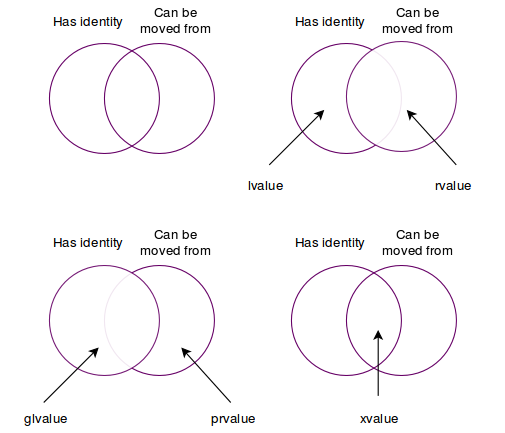
\includegraphics[height=.8\textheight]{valcat.png}

    \scalebox{.7}{(diagrams shamelessly stolen from \href{http://bajamircea.github.io/coding/cpp/2016/04/07/move-forward.html}{\texttt{bajamircea.github.io/coding/cpp/2016/04/07/move-forward.html}})}

\end{frame}

\begin{frame}[fragile]{Value categories with Venn diagrams}
    \begin{center}
        \scalebox{.7}{(diagrams shamelessly stolen from \href{http://bajamircea.github.io/coding/cpp/2016/04/07/move-forward.html}{\texttt{bajamircea.github.io/coding/cpp/2016/04/07/move-forward.html}})}
    \end{center}
    \begin{columns}
        \begin{column}{.7\textwidth}
            \begin{lstlisting}
struct S{ int x; };

S make_S(int x) {
    S s{.x = x};
    return s; // has no name after returning
}

int main() {
    S a = make_S(42); // `a` is an lvalue
                      // initialized with a prvalue

    S b = std::move(a); // prepare to die, `a`!
                        // now `a` became an xvalue

    auto x = a.x; // ERROR: `a` is in an undefined state
    a = make_S(13);
    x = a.x; // fine!
}
            \end{lstlisting}
        \end{column}
        \begin{column}{.25\textwidth}
            \only<1>{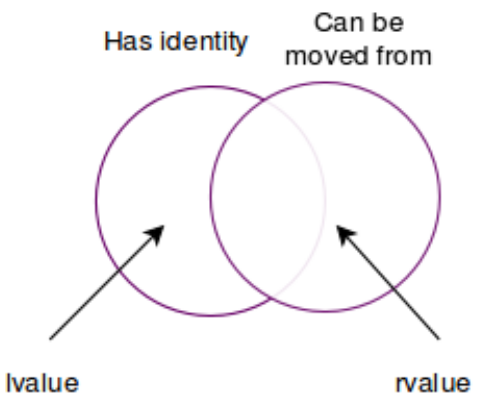
\includegraphics[width=\textwidth]{valcat1.png}}%
            \only<2>{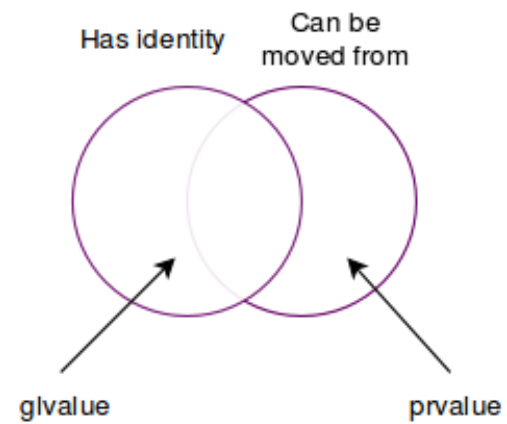
\includegraphics[width=\textwidth]{valcat2.png}}%
            \only<3>{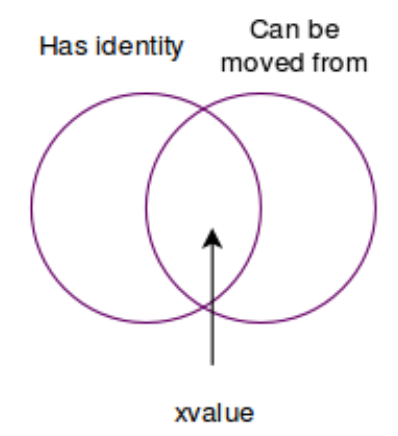
\includegraphics[width=\textwidth]{valcat3.png}}%
        \end{column}
    \end{columns}
\end{frame}

\begin{frame}[fragile]{Binding references to temporaries}
    \begin{center}
        \textbf{\textcolor{vertexDarkRed}{error:}} cannot bind non-const lvalue reference of type \enquote{\texttt{S*\&}} to an rvalue of type \enquote{\texttt{S*}}
    \end{center}
    \begin{columns}
        \begin{column}{.4\textwidth}
            \begin{lstlisting}
template <typename T>
void swap(T& a, T& b) { ... }

int main() {
    S a{1};
    S b{2};
    swap(&a, &b);
}
            \end{lstlisting}
        \end{column}
        \begin{column}{.55\textwidth}
            \begin{itemize}
                \item Memory addresses are always rvalues!
                \item One cannot refer to something that doesn't has a name\ldots
                \item \ldots except it is a const reference (lifetime extension)
            \end{itemize}
        \end{column}
    \end{columns}
\end{frame}

\begin{frame}[plain,noframenumbering]
    \centering
    \scalebox{3}{\texttt{std::move}}
\end{frame}

\begin{frame}[fragile]{\texttt{std::move}}
    \begin{columns}
        \begin{column}{.55\textwidth}
            \inputcpplisting{snippet31}
        \end{column}
        \begin{column}{.4\textwidth}
            \begin{itemize}
                \item \texttt{std::move} creates xvalues
                \item Syntax:
                \begin{itemize}
                    \item lvalue ref.: \texttt{S\&}
                    \item rvalue ref.: \texttt{S\&\&}
                \end{itemize}
            \end{itemize}
        \end{column}
    \end{columns}
\end{frame}

\begin{frame}[fragile]{Q: What is the output of the program?}
    \inputcpplisting{snippet33a}
\end{frame}

\begin{frame}[fragile]{A: \texttt{abac}}
    \begin{columns}
        \begin{column}{.5\textwidth}
            \inputcpplisting{snippet33a}
        \end{column}
        \begin{column}{.45\textwidth}
            \begin{itemize}
                \item \texttt{S s1}: no surprise
                \item \texttt{S s2(s1)}: no surprise
                \item \texttt{S s3(S\{\})}: \href{https://en.cppreference.com/w/cpp/language/copy_elision}{\textit{mandatory} copy elision (initializer is prvalue of the same class type})
                \item \texttt{S s4(std::move(s1))}: forced move construction
            \end{itemize}
        \end{column}
    \end{columns}
\end{frame}

\begin{frame}[fragile]{Q: What is the output of the program?}
    \inputcpplisting{snippet33b}
\end{frame}


\begin{frame}[fragile]{Q: What is the output of the program?}
    \inputcpplisting{snippet33c}
\end{frame}

\begin{frame}[fragile]{Q: What is the output of the program?}
    \begin{columns}
        \begin{column}{.46\textwidth}
            \inputcpplisting{snippet33c}
        \end{column}
        \begin{column}{.49\textwidth}
            \textbf{Compile-time error} (in all three cases)
            \begin{itemize}
                \item \texttt{f(s1)}: ambiguity between \texttt{2} and \texttt{1}
                \item \texttt{f(S\{\})}: ambiguity between \texttt{2} and \texttt{3}
                \item \texttt{f(std::move(s1)}: same as \texttt{f(S{})}
            \end{itemize}

            $\hookrightarrow$ compiler cannot differentiate between copy and reference overloads! (neither lvalue, nor rvalue)
        \end{column}
    \end{columns}
\end{frame}

\begin{frame}[fragile]{Q: What is the output of the program?}
    \inputcpplisting{snippet33d}
\end{frame}

\begin{frame}[fragile]{A: \texttt{23aa}}
    \begin{columns}
        \begin{column}{.46\textwidth}
            \inputcpplisting{snippet33d}
        \end{column}
        \begin{column}{.49\textwidth}
            \begin{itemize}
                \item \texttt{S\&\&}: object that nobody cares about anymore and which will die soon (cf. lifetime extension!)
                \item \texttt{std::move} does not actually kill, but makes the object look like a dying object
            \end{itemize}

            \begin{center}
                \begin{overpic}[width=.8\textwidth]{arya.png}
                    \put(10,10){\color{white}An rvalue has no name} 
                \end{overpic}
            \end{center}
        \end{column}
    \end{columns}

    {\footnotesize \textbf{NB:} an rvalue ref behaves like an lvalue ref except that it can bind to a temporary (an rvalue), whereas one cannot bind a (non const) lvalue ref to an rvalue.}
\end{frame}

\begin{frame}[fragile]{\texttt{std::move}}
    \begin{columns}
        \begin{column}{.55\textwidth}
            \inputcpplisting{snippet34}
        \end{column}
        \begin{column}{.4\textwidth}
            \textbf{So what does \texttt{std::move}?}
            \begin{itemize}
                \item does not \textit{move}
                \item does not destroy
                \item does nothing at all during runtime
                \item \textbf{unconditionally casts} its argument to an rvalue
            \end{itemize}
        \end{column}
    \end{columns}
\end{frame}

\begin{frame}[fragile]{Quick Bench: \href{http://quick-bench.com/7qTMMYSgUJG-lRg-B26ZX77vim0}{\texttt{tinyurl.com/y67sg7to}}}
    \begin{lstlisting}
std::vector<int> x(1000, 42);
std::vector<int> y(1000, 42);
for (auto _ : state) {
    auto tmp = x;
    x = y;
    y = tmp;
    benchmark::DoNotOptimize(x[345] + y[678]);
}
    \end{lstlisting}

    \begin{lstlisting}
std::vector<int> x(1000, 42);
std::vector<int> y(1000, 42);
for (auto _ : state) {
    auto tmp = std::move(x);
    x = std::move(y);
    y = std::move(tmp);
    benchmark::DoNotOptimize(x[345] + y[678]);
}
    \end{lstlisting}
\end{frame}

\begin{frame}{Quick Bench: \href{http://quick-bench.com/7qTMMYSgUJG-lRg-B26ZX77vim0}{\texttt{tinyurl.com/y67sg7to}}}
    \centering

    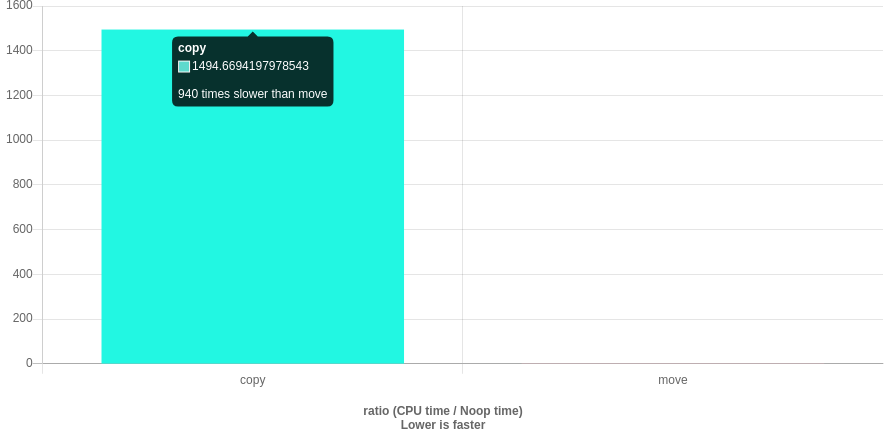
\includegraphics[height=.8\textheight]{benchmark_vec_mv.png}
\end{frame}

\begin{frame}[plain,noframenumbering]
    \centering
    \scalebox{3}{Universal References}
\end{frame}

\section{Universal References}

\begin{frame}[fragile]{Rvalue ref. or no rvalue ref.?}
    Rvalue refs are declared using \enquote{\&\&}: reasonable to assume that the presence of \enquote{\&\&} in a type declaration indicates an rvalue reference?
    \begin{columns}
        \begin{column}{.45\textwidth}
            \begin{lstlisting}[numbers=none]
struct S{};

S&& s = S{};                // (1)

auto&& s2 = s;              // (2)

void f(S&& s);              // (3)

template <typename T>
void f(T&& t);              // (4)

template <typename T>
void f(const T&& t);        // (5)

template <typename T>
void f(std::vector<T>&& v); // (6)
            \end{lstlisting}
        \end{column}
        \begin{column}{.5\textwidth}
            \textbf{Does \enquote{\texttt{\&\&}} mean rvalue reference?}
            \begin{itemize}
                \item \texttt{(1)}: \only<1>{???}
                \item \texttt{(2)}: \only<1>{???}
                \item \texttt{(3)}: \only<1>{???}
                \item \texttt{(4)}: \only<1>{???}
                \item \texttt{(5)}: \only<1>{???}
                \item \texttt{(6)}: \only<1>{???}
            \end{itemize}
        \end{column}
    \end{columns}

    \only<2>{\footnotesize ${}^{\color{vertexDarkRed}\star}$ albeit questionable: \texttt{move} changes object in most cases $\not\leftrightarrow$ \texttt{const}}
\end{frame}

\addtocounter{framenumber}{-1}
\begin{frame}[plain,fragile]
    ${}^{\color{vertexDarkRed}\star}$ albeit questionable: \texttt{move} changes object in most cases $\not\leftrightarrow$ \texttt{const}

    \inputcpplisting{snippet42}
    
    \hfill \scalebox{1.5}{\ldots prints \texttt{A}}

    \begin{center}
        (cf. \href{https://stackoverflow.com/a/28595415}{\texttt{https://stackoverflow.com/a/28595415}})
    \end{center}
\end{frame}

\begin{frame}[fragile]{Universal references}
    \begin{columns}
        \begin{column}{.5\textwidth}
            \textbf{Universal references${}^{\color{vertexDarkRed}\dagger}$}
            \begin{itemize}
                \item Syntax (\texttt{x} is a universal reference):
                \begin{itemize}
                    \item \texttt{auto\&\& x}
                    \item \texttt{template <typename T>} \texttt{f(T\&\& x\ldots}
                \end{itemize}
                \item Rule of thumb: substitute fully qualified type into \texttt{auto} or \texttt{T} and reduce:
                \begin{itemize}
                    \item \texttt{\&\&} $\mapsto$ \texttt{\&\&} 
                    \item \texttt{\&\&\&} $\mapsto$ \texttt{\&} 
                    \item \texttt{\&\&\&\&} $\mapsto$ \texttt{\&\&} 
                \end{itemize}
            \end{itemize}
        \end{column}
        \begin{column}{.45\textwidth}
            \begin{lstlisting}[numbers=none]
std::vector<S> v;
auto&& s = v[0]; // S&&& -> S&

auto&& s2 = S{}; // S&&&& -> S&&
auto&& s3 = s2;  // S&&&  -> S&

// S&&&& -> S&&
auto&& s3 = std::move(s2);
            \end{lstlisting}
        \end{column}
    \end{columns}

    \vspace{5mm}

    \footnotesize ${}^{\color{vertexDarkRed}\dagger}$ \textit{Universal reference}: term introduced by Scott Meyers
\end{frame}

\begin{frame}[fragile]{Q: What is the output of the program?}
    \inputcpplisting{snippet35a}
\end{frame}


\begin{frame}[fragile]{Q: What is the output of the program?}
    \inputcpplisting{snippet37}
\end{frame}


\begin{frame}[fragile]{Q: What is the output of the program?}
    \inputcpplisting{snippet38}
\end{frame}


\begin{frame}[fragile]{Perfect forwarding}
    \centering
    \scalebox{1.5}{How do we fuse these implementations?}

    \begin{lstlisting}
// if `t` is an lvalue of type `S`
S& forward(S& t) {
    return t;
}

// if `t` is an rvalue of type `S`
S&& forward(S& t) { // not `S&&`!
    return std::move(t); // static_cast<S&&>(t)
}
    \end{lstlisting}

    \inputcpplisting{snippet36}
\end{frame}

\begin{frame}[fragile]{Q: What is the output of the program?}
    \inputcpplisting{snippet35b}
\end{frame}

\begin{frame}[fragile]{A: \texttt{abc}}
    \inputcpplisting{snippet35b}
    \textbf{Rule of thumb:} Use \texttt{std::move} for rvalues and \texttt{std::forward} for universal references
\end{frame}

\begin{frame}[fragile]{Q: Why can't we use perfect forwarding here?}
    \inputcpplisting{snippet9}

\end{frame}

\begin{frame}[plain,noframenumbering]
    \centering
    \scalebox{3}{Reading x86-64 Assembly}

    \scalebox{2}{\ldots for fun and profit}
\end{frame}

\section{Reading Assembly for Fun and Profit}

\begin{frame}[fragile]{Function Prologue \& Epilogue}
    \begin{itemize}
        \item Few lines of code at the beginning (\textit{prologue}) and end (\textit{epilogue}) of a function, which \textbf{prepares} (and eventually restores)
        \begin{itemize}
            \item the \textbf{stack} and 
            \item \textbf{registers}
        \end{itemize}
        \item Not part of assembly: \textbf{convention} (defined \& interpreted differently by different OS and compilers)
    \end{itemize}

    \begin{columns}[t]
        \begin{column}{.45\textwidth}
            \textbf{Prologue}
            \begin{lstlisting}[language={}]
push rbp     ; rbp: frame pointer
mov rbp, rsp ; rsp: stack pointer
sub rsp, N
            \end{lstlisting}
            alternatively
            \begin{lstlisting}[language={}]
enter N, 0
            \end{lstlisting}
            (reserve \texttt{N} bytes on stack for local use)
        \end{column}
        \begin{column}{.45\textwidth}
            \textbf{Epilogue}
            \begin{lstlisting}[language={}]
mov rsp, rbp
pop rbp
ret
            \end{lstlisting}
            alternatively
            \begin{lstlisting}[language={}]
leave
ret
            \end{lstlisting}
        \end{column}
    \end{columns}
\end{frame}

\begin{frame}[fragile]{Stack frame for function call}
    \begin{columns}
        \begin{column}{.4\textwidth}
            \begin{itemize}
                \item \texttt{CALL} = \texttt{PUSH} \textit{address of next instruction} + \texttt{JMP} \textit{target}
                \item \texttt{RET} pops return address and transfers control there
                \item pass arguments 1 \ldots 6 in registers (\texttt{rsi}, \texttt{rdx}, \ldots)
            \end{itemize}
        \end{column}
        \begin{column}{.6\textwidth}
            \begin{Verbatim}
┌──────────────┐
│ ...          │
│ 8th Argument │ (rbp + 24)
│ 7th Argument │ (rbp + 16)
├──────────────┤
│ rip          │ (return address)
│ rbp          │ (rbp)
├──────────────┤
│ rbx          │
│ r12          │
│ r13          │ (rsp)
└──────────────┘
            \end{Verbatim}
            (stack frame for function call with 8 arguments and local registers \texttt{rbx}, \texttt{r12} and \texttt{r13})
        \end{column}
    \end{columns}
\end{frame}

\begin{frame}[fragile]{\texttt{lea} vs. \texttt{mov}}
    \begin{columns}
        \begin{column}{.5\textwidth}
            \begin{itemize}
                \item \texttt{lea}: \underline{l}oad \underline{e}ffective \underline{a}ddress
                \item puts memory address from \texttt{src} into the destination \texttt{dest}
                \item Example: \texttt{lea eax, [ebx+8]}
                \begin{itemize}
                    \item put \texttt{[ebx+8]} into \texttt{eax}
                    \item value of \texttt{eax} after instruction: \texttt{0x00403A48}
                \end{itemize}
                \item \ldots whereas: \texttt{mov eax, [ebx+8]}
                \begin{itemize}
                    \item value of \texttt{eax} after instruction: \texttt{0x0012C140}
                \end{itemize}
            \end{itemize}
        \end{column}
        \begin{column}{.5\textwidth}
            \begin{Verbatim}
           ┌──────────────────┐
           │ Registers        │
           ├──────────────────┤
           │ EAX = 0x00000000 │ 
           │ EBX = 0x00403A40 │ 
           └──────────────────┘
           ┌────────────┐
           │ Memory     │
           ├────────────┤
0x00403A40 │ 0x7C81776F │ 
0x00403A44 │ 0x7C911000 │ 
0x00403A48 │ 0x0012C140 │ 
0x00403A4C │ 0x7FFDB000 │ 
           └────────────┘
            \end{Verbatim}
        \end{column}
    \end{columns}
\end{frame}

\begin{frame}[fragile]{Reading assembly for fun and profit}
    \begin{columns}[t]
        \begin{column}{.45\textwidth}
            \inputcpplisting{snippet5a}
            
            \only<2>{%
            \inputasmlisting{snippet5b}}
        \end{column}
        \begin{column}{.45\textwidth}
            \inputasmlisting{snippet5a}
        \end{column}
    \end{columns}
\end{frame}

\begin{frame}[fragile]{Reading assembly for fun and profit}
    \begin{columns}[t]
        \begin{column}{.45\textwidth}
            \inputcpplisting{snippet6a}

            \only<2>{%
            \inputasmlisting{snippet6b}}
        \end{column}
        \begin{column}{.45\textwidth}
            \inputasmlisting{snippet6a}
        \end{column}
    \end{columns}

\end{frame}

\begin{frame}[fragile]{Reading assembly for fun and profit}
    \begin{columns}[t]
        \begin{column}{.45\textwidth}
            \inputcpplisting{snippet1a}
        \end{column}
        \begin{column}{.45\textwidth}
            \inputasmlisting{snippet1a}
        \end{column}
    \end{columns}
\end{frame}


\section{Implicit Costs of \texttt{const\&}}

\begin{frame}[fragile]{Implicit Costs of using \texttt{const\&}}
    \begin{columns}[t]
        \begin{column}{.45\textwidth}
            \inputcpplisting{snippet1a}
        \end{column}
        \begin{column}{.45\textwidth}
            \inputcpplisting{snippet2a}
        \end{column}
    \end{columns}
\end{frame}

\begin{frame}[fragile]{Implicit Costs of using \texttt{const\&}}
    \begin{columns}[t]
        \begin{column}{.45\textwidth}
            \inputasmlisting{snippet1a}
        \end{column}
        \begin{column}{.45\textwidth}
            \inputasmlisting{snippet2a}
        \end{column}
    \end{columns}
\end{frame}

\begin{frame}[fragile]{Implicit Costs of using \texttt{const\&}}
    \begin{columns}[t]
        \begin{column}{.45\textwidth}
            \inputasmlisting{snippet1b}

            \footnotesize
            \only<1>{\textbf{NB \#1:} adjusting \texttt{rsp} in function prologue necessary when function is not a leaf function since callee have to know where to start saving variables on stack. (Adjusting \texttt{rsp} can be ommitted in leaf functions.)}
            \only<2>{\textbf{NB \#2:} Offset \texttt{x} in \texttt{sub rsp, x} is objective of optimizations such as alignment: ABI requires stack to be aligned to 16 bytes.}
        \end{column}
        \begin{column}{.45\textwidth}
            \inputasmlisting{snippet2b}
        \end{column}
    \end{columns}
\end{frame}

\begin{frame}[fragile]{Will it compile?}
    \begin{columns}
        \begin{column}{.45\textwidth}
            \inputcpplisting{snippet39}
        \end{column}
        \begin{column}{.45\textwidth}
            \only<2>{%
            \textbf{\textcolor{vertexDarkRed}{No!}}
            \begin{itemize}
                \item Constructor takes by reference
                \item References to automatic storage objects are not constant expressions!
                \item Solutions?
            \end{itemize}}
        \end{column}
    \end{columns}

    \vspace{1cm}

    \begin{lstlisting}
template <std::size_t N>
constexpr span(const std::array<value_type, N>& arr) noexcept;
    \end{lstlisting}
    \href{https://en.cppreference.com/w/cpp/container/span/span}{\texttt{cppreference.com/w/cpp/container/span/span}}
\end{frame}

\begin{frame}[fragile]{Will it compile?}
    \inputcpplisting{snippet40}
\end{frame}

\begin{frame}[fragile]{Nota bene \ldots}
    this will work though, since reference / pointer does not \textit{escape} constant expression \ldots
    \inputcpplisting{snippet41}
\end{frame}

\begin{frame}[plain,noframenumbering]
    \centering
    \scalebox{5}{PART II}
\end{frame}

\begin{frame}[plain,noframenumbering]
    \centering
    \scalebox{3}{Dangling References}
\end{frame}

\section{Dangling References}

\begin{frame}[fragile]{Will it compile?}
    \inputcpplisting{snippet22a}

\end{frame}

\begin{frame}[fragile]{Will it invoke undefined behavior?}
    \inputcpplisting{snippet22b}

    \hfill \ldots binding a reference to a temporary???
\end{frame}

\begin{frame}[fragile]{Temporary object lifetime extension}
    \inputcpplisting{snippet22b}

    \href{https://en.cppreference.com/w/cpp/language/lifetime}{\texttt{cppreference.com}: \enquote{The lifetime of a temporary object may be extended by binding to a const lvalue reference or to an rvalue reference (since C++11).}}
\end{frame}

\begin{frame}[fragile]{Q: What is the output of the program?}
    \inputcpplisting{snippet29}
\end{frame}

\begin{frame}[fragile]{A: \texttt{a1b1a2xb2}}
    \begin{columns}
        \begin{column}{.55\textwidth}
            \inputcpplisting{snippet29}
        \end{column}
        \begin{column}{.4\textwidth}
            \textbf{Dangling reference!!!}
            \begin{itemize}
                \item lifetime extension only for result of the temporary expression, \textbf{not any sub-expression}
                \item use \href{https://clang.llvm.org/docs/AddressSanitizer.html}{address sanitizer}!    
            \end{itemize}
        \end{column}
    \end{columns}
\end{frame}

\begin{frame}[plain,noframenumbering]
    \centering
    \scalebox{2.}{contrived?}
\end{frame}

\begin{frame}[fragile]{Reference lifetime extension}
    \begin{center}
        \scalebox{.7}{(derived from \href{https://abseil.io/tips/107}{\texttt{abseil.io}: Tip of the Week \#107: \enquote{Reference Lifetime Extension})}}
    \end{center}

    \begin{lstlisting}
std::vector<std::string_view> explode(const std::string& s);

for (std::string_view s: explode(str_cat("oo", "ps"))) { // WRONG!
    [...]
    \end{lstlisting}
\end{frame}

\begin{frame}[fragile]{Q: What is the output of the program?}
    \begin{columns}
        \begin{column}{.45\textwidth}
            \inputcpplisting{snippet30}
        \end{column}
        \begin{column}{.5\textwidth}
            \only<2>{%
            \textbf{Dangling reference!!!}
            \begin{itemize}
                \item \texttt{std::vector} needs to reallocate all the space the second time an element is pushed 
                \item use \href{https://clang.llvm.org/docs/AddressSanitizer.html}{address sanitizer}!    
            \end{itemize}}
        \end{column}
    \end{columns}
\end{frame}

\begin{frame}[plain,noframenumbering]
    \centering
    \scalebox{3}{\texttt{std::move} in the wild}
\end{frame}

\section{\texttt{std::move} in the wild}

\begin{frame}[fragile]{Moving \texttt{std::string}}
    \centering
    \scalebox{.7}{(derived from \href{https://youtu.be/oTMSgI1XjF8}{CppCon 2019: \textit{Ben Deane} \enquote{Everyday Efficiency: In-Place Construction (Back to Basics?)})}}

    \begin{lstlisting}
static void cp_small_str(benchmark::State& state) {
    for (auto _ : state) {
        std::string original("small");
        benchmark::DoNotOptimize(original);
        std::string copied = original;
        benchmark::DoNotOptimize(copied);
    }
}
BENCHMARK(cp_small_str);
    \end{lstlisting}

    \begin{lstlisting}
static void mv_small_str(benchmark::State& state) {
    for (auto _ : state) {
        std::string original("small");
        benchmark::DoNotOptimize(original);
        std::string moved = std::move(original);
        benchmark::DoNotOptimize(moved);
    }
}
BENCHMARK(mv_small_str);
    \end{lstlisting}
\end{frame}

\begin{frame}[fragile]{Moving \texttt{std::string}}
    \centering
    \scalebox{.7}{(derived from \href{https://youtu.be/oTMSgI1XjF8}{CppCon 2019: \textit{Ben Deane} \enquote{Everyday Efficiency: In-Place Construction (Back to Basics?)})}}

    \begin{lstlisting}
static void cp_long_str(benchmark::State& state) {
    for (auto _ : state) {
        std::string original("this is too long for short string optimization");
        benchmark::DoNotOptimize(original);
        std::string copied = original;
        benchmark::DoNotOptimize(copied);
    }
}
BENCHMARK(cp_long_str);
    \end{lstlisting}

    \begin{lstlisting}
static void mv_long_str(benchmark::State& state) {
    for (auto _ : state) {
        std::string original("this is too long for short string optimization");
        benchmark::DoNotOptimize(original);
        std::string moved = std::move(original);
        benchmark::DoNotOptimize(moved);
    }
}
BENCHMARK(mv_long_str);
    \end{lstlisting}
\end{frame}

\begin{frame}{Moving \texttt{std::string}}
    \centering
    \scalebox{1.5}{Quick Bench result}

    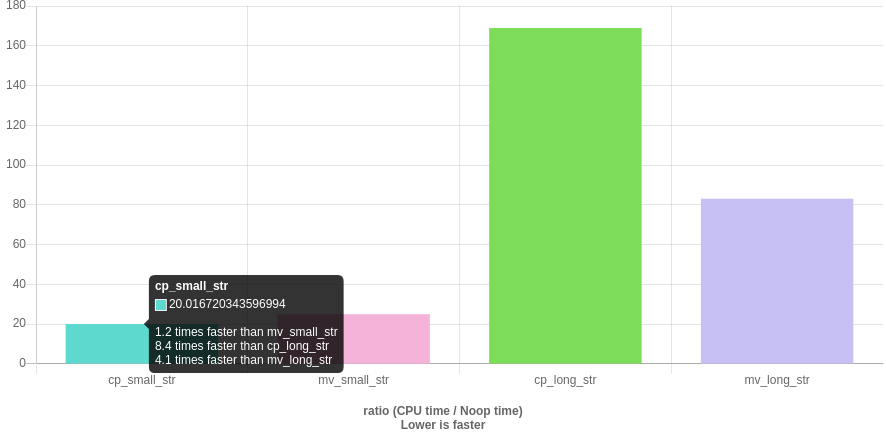
\includegraphics[width=.9\textwidth]{benchmark_str_cp_mv.png}

    Quick Bench: \href{http://quick-bench.com/l_4Ith4ZvZbSE0UIfIQXVpkg84A}{\texttt{tinyurl.com/yybmdngv}}
\end{frame}

\begin{frame}[fragile]{Moving \texttt{std::string}}
    \centering

    \begin{columns}[t]
        \begin{column}{.45\textwidth}
            \begin{block}{Copy small \texttt{std::string}}
                \begin{enumerate}
                    \item copy stack allocated data
                \end{enumerate}
            \end{block}
        \end{column}
        \begin{column}{.45\textwidth}
            \begin{block}{Move small \texttt{std::string}}
                \begin{enumerate}
                    \item copy stack allocated data
                    \item set string length of moved string to zero
                \end{enumerate}
            \end{block}
        \end{column}
    \end{columns}

    \vspace{5mm}

    \begin{center}
        \scalebox{1.5}{$\hookrightarrow$ moving is not necessarily better than copying!}
    \end{center}
\end{frame}

\begin{frame}[fragile]{Moving \texttt{std::map}}
    \textbf{Did they forget to mark the move ctor \texttt{noexcept}?} \only<2>{\textcolor{vertexDarkRed}{No!}}

    \begin{columns}[t]
        \begin{column}{.45\textwidth}
            \begin{lstlisting}[numbers=none]
// since C++11
std:map(const std:map&&)

// until C++17
std:map& operator(std:map&&)

// since C++17
std:map& operator(std:map&&) noexcept
            \end{lstlisting}
        \end{column}
        \begin{column}{.5\textwidth}
            \begin{itemize}
                \item<2> Move ctor needs to allocate new sentinel node, because moved from container must still be a valid container (albeit in an unspecified state)
                \item<2> Move assignment can swap, thus no need to allocate
            \end{itemize}
        \end{column}
    \end{columns}

    \only<2>{%
    \begin{center}
        \scalebox{1.5}{$\hookrightarrow$ move ctor of \texttt{std::map} allocates heap space!}

        \scalebox{.8}{(Billy O'Neal: \href{https://twitter.com/MalwareMinigun/status/1165310509022736384}{\texttt{twitter.com/MalwareMinigun/status/1165310509022736384})}}
    \end{center}}
\end{frame}

\begin{frame}[fragile]{Moving \texttt{std::map}}
    \begin{lstlisting}
static void rvo(benchmark::State& state) {
    for (auto _ : state) {
        auto m = []() -> std::map<int, int> {
            std::map<int, int> m{{0, 42}};
            return m;
        }();
        benchmark::DoNotOptimize(m);
    }
}
BENCHMARK(rvo);
    \end{lstlisting}

    \begin{lstlisting}
static void fmove(benchmark::State& state) {
    for (auto _ : state) {
        auto m = []() -> std::map<int, int> {
            std::map<int, int> m{{0, 42}};
            return std::move(m);
        }();
        benchmark::DoNotOptimize(m);
    }
}
BENCHMARK(fmove);
    \end{lstlisting}
\end{frame}
\begin{frame}[fragile]{Moving \texttt{std::map}}
    \begin{lstlisting}
static void copy(benchmark::State& state) {
    for (auto _ : state) {
        std::map<int, int> m{{0, 42}};
        benchmark::DoNotOptimize(m);
        auto m2 = m;
        benchmark::DoNotOptimize(m2);
    }
}
BENCHMARK(copy);
    \end{lstlisting}
\end{frame}

\begin{frame}{Moving \texttt{std::map}}
    \centering
    \scalebox{1.5}{Quick Bench result}

    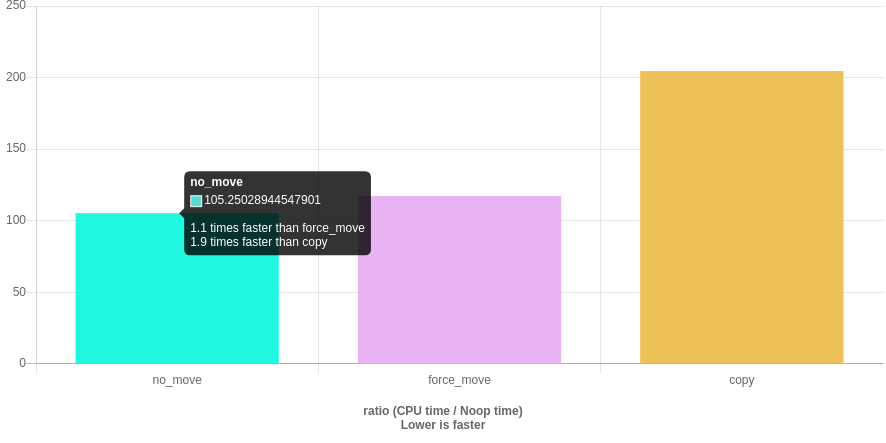
\includegraphics[width=.9\textwidth]{benchmark_map_mv.png}

    Quick Bench: \href{http://quick-bench.com/7L-__vxvraDDacztJoalrjBrMUA}{\texttt{tinyurl.com/y57egvjp}}
\end{frame}

\begin{frame}[plain,noframenumbering]
    \centering
    \scalebox{5}{Why?}
\end{frame}

\begin{frame}[fragile]{Does this code bother anyone?}
    \inputcpplisting{snippet3}
\end{frame}

\begin{frame}[plain,noframenumbering]
    \centering
    \scalebox{2}{Interlude}

    \scalebox{3}{What happens on \texttt{return}?}
\end{frame}

\section{What Happens on \texttt{return}?}

\begin{frame}[fragile]{Will it compile?}
    \inputcpplisting{snippet8}
\end{frame}


\begin{frame}[fragile]{Implicit conversion to the function return type}
    \begin{columns}
        \begin{column}{.55\textwidth}
            \textbf{Implicit conversion}
            \begin{itemize}
                \item \ldots if ctor is \textbf{not} marked \texttt{explicit}
                \item Examples: 
                \begin{itemize}
                    \item \href{https://en.cppreference.com/w/cpp/utility/optional/optional}{\texttt{std::optional(T\&\&)}}
                    \item \href{https://en.cppreference.com/w/cpp/string/basic_string/basic_string}{\texttt{std::string(const char*)}}
                \end{itemize}
            \end{itemize}
        \end{column}
        \begin{column}{.35\textwidth}
            \inputcpplisting{snippet27}
        \end{column}
    \end{columns}
\end{frame}

\begin{frame}[fragile]{Q: What is the output of the program?}
    \begin{center}
        Compiler flags: \texttt{-std=c++14 -fno-elide-constructors}
    \end{center}

    \inputcpplisting{snippet4a}
\end{frame}


\begin{frame}[fragile]{Q: What is the output of the program?}
    \begin{center}
        Compiler flags: \texttt{-std=c++17}
    \end{center}

    \inputcpplisting{snippet4b}
\end{frame}


\begin{frame}[plain,noframenumbering]
    \centering
    \scalebox{5}{\only<1>{Why?}
    }

    \only<2>{Ben Deane: \enquote{Perhaps the most important optimization the compiler does}}
\end{frame}

\begin{frame}{Copy Elision}
    \begin{columns}
        \begin{column}{.45\textwidth}
            \inputcpplisting{snippet10}
        \end{column}
        \begin{column}{.5\textwidth}
            Mandatory elision of copy/move operations since \texttt{C++17}):
            \begin{itemize}
                \item Return statement: when operand is a \texttt{prvalue} of same class type as return type
                \item Initialization of a variable: when initializer expression is a \texttt{prvalue} of same class type as the variable type
            \end{itemize}
        \end{column}
    \end{columns}
    \ldots even if the copy/move constructor and the destructor has observable side-effects!
    \vspace{.5cm}

    \centering
    \scalebox{1.5}{\textbf{Rule of thumb: avoid naming return values}}
\end{frame}

\section{RVO in Depth}

\begin{frame}[plain,noframenumbering]
    \centering
    \scalebox{3}{RVO in Depth}
\end{frame}

\begin{frame}[fragile]{\texttt{C++} Objects in Assembly}
    \begin{columns}[t]
        \begin{column}{.45\textwidth}
            \inputcpplisting{snippet20}
        \end{column}
        \begin{column}{.45\textwidth}
            \begin{lstlisting}[language={},morekeywords={rdi},numbers=none]
  | main:
14|   push rbp
14|   mov rbp, rsp
14|   sub rsp, 16
14|   mov dword ptr [rbp - 4], 0
15|   lea rdi, [rbp - 16]
15|   mov esi, 1
15|   mov edx, 2
15|   mov ecx, 3
15|   call S::S(int, int, int)
16|   lea rdi, [rbp - 16]
16|   call S::sum()
16|   mov dword ptr [rbp - 4], eax
17|   lea rdi, [rbp - 16]
17|   call S::~S()
17|   mov eax, dword ptr [rbp - 4]
17|   add rsp, 16
17|   pop rbp
17|   ret
            \end{lstlisting}
        \end{column}
    \end{columns}
\end{frame}

\begin{frame}[fragile]{\texttt{C++} Objects in Assembly}
    \begin{columns}[t]
        \begin{column}{.45\textwidth}
            \inputcpplisting{snippet20}
        \end{column}
        \begin{column}{.45\textwidth}
            \begin{lstlisting}[language={},morekeywords={rdi},numbers=none]
  | S::S(int, int, int):
 5|   push rbp
 5|   mov rbp, rsp
 5|   mov qword ptr [rbp - 8], rdi
 5|   mov dword ptr [rbp - 12], esi
 5|   mov dword ptr [rbp - 16], edx
 5|   mov dword ptr [rbp - 20], ecx
 5|   mov rax, qword ptr [rbp - 8]
 5|   mov ecx, dword ptr [rbp - 12]
 5|   mov dword ptr [rax], ecx
 5|   mov ecx, dword ptr [rbp - 16]
 5|   mov dword ptr [rax + 4], ecx
 5|   mov ecx, dword ptr [rbp - 20]
 5|   mov dword ptr [rax + 8], ecx
 5|   pop rbp
 5|   ret
            \end{lstlisting}
        \end{column}
    \end{columns}
\end{frame}

\begin{frame}[fragile]{\texttt{C++} Objects in Assembly}
    \begin{columns}[t]
        \begin{column}{.45\textwidth}
            \inputcpplisting{snippet20}
        \end{column}
        \begin{column}{.45\textwidth}
            \begin{lstlisting}[language={},morekeywords={rdi},numbers=none]
  | S::sum():
 9|   push rbp
 9|   mov rbp, rsp
 9|   mov qword ptr [rbp - 8], rdi
 9|   mov rax, qword ptr [rbp - 8]
10|   mov ecx, dword ptr [rax]
10|   add ecx, dword ptr [rax + 4]
10|   add ecx, dword ptr [rax + 8]
10|   mov eax, ecx
10|   pop rbp
10|   ret
            \end{lstlisting}
        \end{column}
    \end{columns}
\end{frame}

\begin{frame}[fragile]{RVO in Assembly}
    \begin{columns}[t]
        \begin{column}{.45\textwidth}
            \inputcpplisting{snippet7}
        \end{column}
        \begin{column}{.45\textwidth}
            \begin{lstlisting}[language={},morekeywords={rdi},numbers=none]
# g92 -fno-elide-constructors
  | g():
  |   [...]
14|   lea rax, [rbp-20]
14|   mov rdi, rax
14|   call f()
14|   lea rdx, [rbp-20]
14|   lea rax, [rbp-24]
14|   mov rsi, rdx
14|   mov rdi, rax
14|   call S::S(S&&)
14|   lea rax, [rbp-20]
14|   mov rdi, rax
14|   call S::~S()
15|   mov ebx, DWORD PTR [rbp-24]
14|   lea rax, [rbp-24]
14|   mov rdi, rax
14|   call S::~S()
15|   mov eax, ebx
  |   [...]      
            \end{lstlisting}
        \end{column}
    \end{columns}
\end{frame}

\begin{frame}[fragile]{RVO in Assembly}
    \begin{columns}[t]
        \begin{column}{.45\textwidth}
            \inputcpplisting{snippet7}
        \end{column}
        \begin{column}{.45\textwidth}
            \begin{lstlisting}[language={},morekeywords={rdi},numbers=none]
# g92 -fno-elide-constructors
  | f():
  |   [...]
 9|   mov QWORD PTR [rbp-24], rdi
10|   lea rax, [rbp-4]
10|   mov esi, 42
10|   mov rdi, rax
10|   call S::S(int)
10|   lea rdx, [rbp-4]
10|   mov rax, QWORD PTR [rbp-24]
10|   mov rsi, rdx
10|   mov rdi, rax
10|   call S::S(S&&)
10|   lea rax, [rbp-4]
10|   mov rdi, rax
10|   call S::~S()
  |   [...]      
            \end{lstlisting}
        \end{column}
    \end{columns}
\end{frame}

\begin{frame}[fragile]{RVO in Assembly}
    \begin{columns}[t]
        \begin{column}{.45\textwidth}
            \begin{lstlisting}[language={},morekeywords={rdi}]
# g92 -fno-elide-constructors
f():
  [...]
  mov QWORD PTR [rbp-24], rdi
  lea rax, [rbp-4]
  mov esi, 42
  mov rdi, rax
  call S::S(int)
  lea rdx, [rbp-4]
  mov rax, QWORD PTR [rbp-24]
  mov rsi, rdx
  mov rdi, rax
  call S::S(S&&)
  lea rax, [rbp-4]
  mov rdi, rax
  call S::~S()
  nop
  mov rax, QWORD PTR [rbp-24]
  leave
  ret
            \end{lstlisting}
        \end{column}
        \begin{column}{.45\textwidth}
            \begin{lstlisting}[language={},morekeywords={rdi}]
# g92
f():
  [...]
  mov QWORD PTR [rbp-8], rdi
  mov rax, QWORD PTR [rbp-8]
  mov esi, 42
  mov rdi, rax
  call S::S(int)
  mov rax, QWORD PTR [rbp-8]
  leave
  ret
            \end{lstlisting}
        \end{column}
    \end{columns}
\end{frame}

\begin{frame}[fragile]{RVO in Assembly}
    \begin{columns}[t]
        \begin{column}{.45\textwidth}
            \begin{lstlisting}[language={},morekeywords={rdi}]
# g92 -fno-elide-constructors
g():
  [...]
  lea rax, [rbp-20]
  mov rdi, rax
  call f()
  lea rdx, [rbp-20]
  lea rax, [rbp-24]
  mov rsi, rdx
  mov rdi, rax
  call S::S(S&&)
  lea rax, [rbp-20]
  mov rdi, rax
  call S::~S()
  mov ebx, DWORD PTR [rbp-24]
  lea rax, [rbp-24]
  mov rdi, rax
  call S::~S()
  mov eax, ebx
  [...]      
            \end{lstlisting}
        \end{column}
        \begin{column}{.45\textwidth}
            \begin{lstlisting}[language={},morekeywords={rdi}]
# g92
g():
  [...]
  lea rax, [rbp-20]
  mov rdi, rax
  call f()
  mov ebx, DWORD PTR [rbp-20]
  lea rax, [rbp-20]
  mov rdi, rax
  call S::~S()
  mov eax, ebx
            \end{lstlisting}
        \end{column}
    \end{columns}
\end{frame}

\begin{frame}[fragile]{(N)RVO or no (N)RVO?}
    \inputcpplisting{snippet21}
    \begin{itemize}
        \item \texttt{f1}: \only<1>{???}
        \item \texttt{f2}: \only<1>{???}
        \item \texttt{f3}: \only<1>{???}
        \item \texttt{f4}: \only<1>{???}
    \end{itemize}
\end{frame}

\begin{frame}[fragile]{(N)RVO or no (N)RVO?}
    \inputcpplisting{snippet25}
    \begin{itemize}
        \item \texttt{f1}: \only<1>{???}
        \item \texttt{f2}: \only<1>{???}
        \item \texttt{f3}: \only<1>{???}
    \end{itemize}
\end{frame}

\begin{frame}[fragile]{(N)RVO or no (N)RVO?}
    \inputcpplisting{snippet23}

\end{frame}

\begin{frame}[fragile]{(N)RVO or no (N)RVO?}
    \inputcpplisting{snippet26}
    \begin{itemize}
        \item \texttt{f1}: \only<1>{???}
        \only<2>{RVO: type of ternary is prvalue}
        \item \texttt{f2}: \only<1>{???}
    \end{itemize}

\end{frame}

\begin{frame}[fragile]{(N)RVO or no (N)RVO?}
    \inputcpplisting{snippet24}
    \begin{itemize}
        \item \texttt{g1}: \only<1>{???}
        \item \texttt{g2}: \only<1>{???}
        \item \texttt{g3}: \only<1>{???}
        \item \texttt{g4}: \only<1>{???}
    \end{itemize}
\end{frame}

\begin{frame}[fragile]{(N)RVO or no (N)RVO?}
    \begin{center}
        \scalebox{.7}{(derived from \href{https://youtu.be/ZxWjii99yao}{CppCon 2019: \textit{Jason Turner} \enquote{Great C++ is\_trivial}})}
    \end{center}

    \textbf{No (N)RVO in any of these examples!}
    \begin{lstlisting}
S g1() { auto [s1, s2] = f(); return s1; } // copy
S g2() { auto&& [s1, s2] = f(); return s1; } // copy: no implicit move yet (?)
S g3() { auto [s1, s2] = f(); return std::move(s1); } // move
S g4() { auto&& [s1, s2] = f(); return std::move(s1); } // move
    \end{lstlisting}
    
    \hfill \ldots \texttt{return std::move} is not always bad

    \textbf{Why?} Structured bindings:
    \begin{itemize}
        \item Creation of temporary object \texttt{e}
        \item Like a reference: structured binding is an alias into \texttt{e}
    \end{itemize}
\end{frame}

\begin{frame}{Implicit move}
    \begin{center}
        \scalebox{1.5}{\texttt{return std::move} is not yet necessarily a code smell}

        (use \texttt{-Wpessimizing-move})
    \end{center}

    \href{https://en.cppreference.com/w/cpp/language/return}{\textbf{Automatic move from local variables and parameters \underline{if}:}}
    \begin{itemize}
        \item return expression names a variable whose type is either
        \begin{itemize}
            \item an object type or (since \texttt{C++11})
            \item an rvalue reference to object type (since \texttt{C++20}${}^{\textcolor{vertexDarkRed}\star}$)
        \end{itemize}
        \item \ldots and that variable is declared
        \begin{itemize}
            \item in the body or
            \item as a parameter of
        \end{itemize}
        \item \ldots the innermost enclosing function or lambda expression
    \end{itemize}

    ${}^{\textcolor{vertexDarkRed}\star}$ \scalebox{.8}{\href{http://www.open-std.org/jtc1/sc22/wg21/docs/papers/2019/p1825r0.html}{\texttt{P1825R0}} (not yet implemented in GCC or Clang: \href{https://en.cppreference.com/w/cpp/compiler_support}{cppreference.com/w/cpp/compiler\_support})}
\end{frame}

\begin{frame}[plain,noframenumbering]
    \centering
    \scalebox{3}{Perfect Backwarding}
\end{frame}

\section{Perfect Backwarding}

\begin{frame}[fragile]{Forwarding Values and Preserving Value Category}
    \centering

    \scalebox{.7}{(derived from \href{https://youtu.be/hwT8K3-NH1w}{CppCon 2018: \textit{Hayun Ezra Chung} \enquote{Forwarding Values... and Backwarding Them Too?})}}

    \only<1>{\inputcpplisting{snippet11a}}%
    \only<2>{\inputcpplisting{snippet11b}}%
    \only<3>{\inputcpplisting{snippet11c}}%
\end{frame}

\begin{frame}[fragile]{Backwarding Values and Preserving Value Category}
    \only<1>{\inputcpplisting{snippet18a}}%
    \only<2>{\inputcpplisting{snippet18b}}%
\end{frame}

\begin{frame}[fragile]{Backwarding Values and Preserving Value Category}
    \textbf{Q:} Why is this a bad idea?
    \begin{lstlisting}
auto&& visit(auto visitor) {
    auto&& result = visitor(resource);
    return result;
}
    \end{lstlisting}
    
    \only<2>{%
    \textbf{A:} Dangling reference for

    \centering
    \texttt{visit([](Resource\& r) -> Resource \{ return r; \}));}

    \vspace{.5cm}

    \begin{center}
        \scalebox{1.5}{\texttt{auto\&\&} is always a reference!}
    \end{center}}
\end{frame}

\begin{frame}[fragile]{Backwarding Values and Preserving Value Category}
    \only<1>{\inputcpplisting{snippet12a}}%
    \only<2>{\inputcpplisting{snippet12b}}
\end{frame}

\begin{frame}[fragile]{Backwarding Values and Preserving Value Category}
    \only<1>{\inputcpplisting{snippet13a}}%
    \only<2>{\inputcpplisting{snippet13b}}
\end{frame}

\begin{frame}[fragile]{Backwarding Values and Preserving Value Category}
    \centering
    \only<1>{\inputcpplisting{snippet14a}}%
    \only<2,3>{%
        \only<3>{\textbf{\textcolor{vertexDarkRed}{error:}} cannot bind rvalue reference of type \enquote{Resource\&\&} to lvalue of type \enquote{Resource}}%
        \inputcpplisting{snippet14b}%
    }%
    \only<4>{\inputcpplisting{snippet14c}}
\end{frame}

\begin{frame}[fragile]{Backwarding Values and Preserving Value Categroy}
    \centering
    \scalebox{1.5}{How do we fuse these implementations?}

    \begin{lstlisting}
Resource visit(auto visitor) {
    Resource result = visitor(resource);
    return result;
}

Resource& visit(auto visitor) {
    Resource& result = visitor(resource);
    return result;
}

Resource&& visit(auto visitor) {
    Resource&& result = visitor(resource);
    return static_cast<Resource&&>(result);
}
    \end{lstlisting}

    \begin{lstlisting}
Target(rm.visit([](Resource& r) -> Resource { return r; }));
Target(rm.visit([](Resource& r) -> Resource& { return r; }));
Target(rm.visit([](Resource& r) -> Resource&& { return std::move(r); }));
    \end{lstlisting}
\end{frame}

\begin{frame}[fragile]{Backwarding Values and Preserving Value Categroy}
    \centering
    \scalebox{1.5}{How do we fuse these implementations?}

    \begin{lstlisting}
Resource visit(auto visitor) {
    Resource result = visitor(resource);
    return result;
}

Resource& visit(auto visitor) {
    Resource& result = visitor(resource);
    return result;
}

Resource&& visit(auto visitor) {
    Resource&& result = visitor(resource);
    return static_cast<Resource&&>(result);
}
    \end{lstlisting}

    \begin{lstlisting}
decltype(auto) visit(auto visitor) {
    decltype(auto) result = visitor(resource);
    return static_cast<decltype(result)>(result);
}
    \end{lstlisting}
\end{frame}

\begin{frame}[fragile,plain,noframenumbering]
    \centering
    \scalebox{.7}{(derived from \href{https://youtu.be/hwT8K3-NH1w}{CppCon 2018: \textit{Hayun Ezra Chung} \enquote{Forwarding Values... and Backwarding Them Too?})}}

    \inputcpplisting{snippet15}
\end{frame}

\begin{frame}[plain,noframenumbering]
    \centering
    \scalebox{5.}{\color{vertexDarkRed}$*$}
\end{frame}

\begin{frame}[fragile]{Q: What is the output of the program?}
    \inputcpplisting{snippet16a}
\end{frame}


\begin{frame}[fragile]{Q: What is the output of the program?}
    \inputcpplisting{snippet16b}
\end{frame}


\begin{frame}[fragile]{Missing (N)RVO}
    \begin{lstlisting}
struct Resource {
    [...]
    Resource(const Resource&) { std::cout << 'a'; }
};

Resource visit(auto visitor) {
    Resource result = visitor(resource);
    return static_cast<Resource>(result);
}
    \end{lstlisting}

    \textbf{Neither RVO nor NRVO!}
    \begin{itemize}
        \item \texttt{static\_cast} is not the name of a variable (c-style cast does not work either)
        \item compiler cannot elide observable side effects of copy construction
        \item \enquote{Solution}
        \begin{itemize}
            \item remove explicit cast, or
            \item remove side effect (\texttt{std::cout})
        \end{itemize}
    \end{itemize}
\end{frame}

\begin{frame}[fragile]{Missing (N)RVO}
    \begin{lstlisting}
template <typename T>
decltype(auto) visit(T visitor) {
    decltype(auto) result = visitor(resource);
    if constexpr (std::is_same_v<decltype(result), Resource&&>) {
        return std::move(result);
    } else {
        return result;
    }
}
    \end{lstlisting}

    \hfill \ldots works for GCC (without \texttt{auto} concept), not for Clang though
\end{frame}

\begin{frame}[fragile]{Missing (N)RVO}
    \begin{lstlisting}
template <typename T>
static constexpr bool returns_rref = std::is_same_v<std::invoke_result_t<T, Resource&>, Resource&&>;

template <typename T, std::enable_if_t<returns_rref<T>, int> = 0>
decltype(auto) visit(T visitor) {
    decltype(auto) result = visitor(resource);
    return std::move(result);
}

template <typename T, std::enable_if_t<not returns_rref<T>, int> = 0>
decltype(auto) visit(T visitor) {
    decltype(auto) result = visitor(resource);
    return result;
}
    \end{lstlisting}

    \hfill \ldots still, no NRVO with Clang but this time due to the deduced return type!
\end{frame}

\begin{frame}[fragile]{Missing (N)RVO}
    \begin{lstlisting}
template <typename T>
static constexpr bool returns_rref = std::is_same_v<std::invoke_result_t<T, Resource&>, Resource&&>;

template <typename T, std::enable_if_t<returns_rref<T>, int> = 0>
decltype(auto) visit(T visitor) {
    decltype(auto) result = visitor(resource);
    return std::move(result);
}

template <typename T, std::enable_if_t<not returns_rref<T>, int> = 0>
auto visit(T visitor) -> decltype(visitor(resource)) {
    decltype(auto) result = visitor(resource);
    return result;
}
    \end{lstlisting}

    \hfill \ldots now works for GCC and Clang!
\end{frame}

\begin{frame}[fragile,plain,noframenumbering]
    \inputcpplisting{snippet17}
\end{frame}

\begin{frame}[fragile,plain,noframenumbering]
    \scalebox{3.}{More things that don't work}
\end{frame}

\begin{frame}[fragile]{Missing (N)RVO}
    \inputcpplisting{snippet19a}

    \hfill \ldots works with GCC, fails with Clang
\end{frame}


\begin{frame}[fragile]{Missing (N)RVO}
    \inputcpplisting{snippet19b}

    \hfill \ldots works with Clang, fails with GCC
\end{frame}

\begin{frame}[fragile]{Missing (N)RVO}
    \inputcpplisting{snippet19c}

    \hfill \ldots fails with GCC and Clang
\end{frame}

\begin{frame}{Conclusion}
    \begin{center}
        \scalebox{.7}{(shamelessly copied from \href{https://youtu.be/hwT8K3-NH1w}{CppCon 2018: \textit{Hayun Ezra Chung} \enquote{Forwarding Values... and Backwarding Them Too?})}}
    \end{center}
    
    \textbf{Forwarding}
    \begin{itemize}
        \item Parameter Type: \texttt{T\&\&}
        \item Function Argument: \texttt{std::forward<E>(e)}
        \item Alternatively: \texttt{static\_cast<decltype(e)\&\&>(e)}
    \end{itemize}

    \textbf{Backwarding}
    \begin{itemize}
        \item Parameter Type: \texttt{decltype(auto)}
        \item Function Argument: \texttt{decltype(e)(e)}
        \item Alternatively: \texttt{static\_cast<decltype(e)>(e)}$^*$
    \end{itemize}
\end{frame}

\include{part3_pv}}{
\begin{frame}[plain,noframenumbering]
    \centering
    \scalebox{5}{PART I}
\end{frame}

\begin{frame}[plain,noframenumbering]
    \centering
    \scalebox{3}{Understanding References}
\end{frame}

\section{Understanding References}

\begin{frame}[fragile]{Q: What is the output of the programs?}
    \begin{columns}[t]
        \begin{column}{.45\textwidth}
% REMOVE_FOR_PRINT {
        \only<2>{A: \texttt{12}}
% REMOVE_FOR_PRINT }

    \begin{lstlisting}[language=python]
#!/usr/bin/env python3

class S:
    def __init__(self, x):
        self.x = x

def swap(a, b):
    b, a = a, b

if __name__ == '__main__':
    a, b = S(1), S(2)
    swap(a, b)
    print(f'{a.x}{b.x}')
    \end{lstlisting}
        \end{column}
        \begin{column}{.45\textwidth}
% REMOVE_FOR_PRINT {
            \only<2>{A: \texttt{22}}
% REMOVE_FOR_PRINT }

            \inputcpplisting{snippet28a}
        \end{column}
    \end{columns}
\end{frame}

\begin{frame}[fragile]{Q: What is the output of the program?}
    \inputcpplisting{snippet28b}
\end{frame}

% REMOVE_FOR_PRINT {
\addtocounter{framenumber}{-1}
\begin{frame}[fragile]{A: \texttt{21}}
    \inputcpplisting{snippet28b}
\end{frame}
% REMOVE_FOR_PRINT }

\begin{frame}[fragile]{Q: What is the output of the program?}
    \inputcpplisting{snippet28c}
\end{frame}

% REMOVE_FOR_PRINT {
\addtocounter{framenumber}{-1}
\begin{frame}[fragile]{A: \texttt{aacc22}}
    \inputcpplisting{snippet28c}
\end{frame}
% REMOVE_FOR_PRINT }

\begin{frame}[fragile]{Q: What is the output of the program?}
    \inputcpplisting{snippet28d}
\end{frame}

% REMOVE_FOR_PRINT {
\addtocounter{framenumber}{-1}
\begin{frame}[fragile]{A: \texttt{aabcc21}}
    \inputcpplisting{snippet28d}
\end{frame}
% REMOVE_FOR_PRINT }

\begin{frame}[fragile]{Q: What is the output of the program?}
    \inputcpplisting{snippet28e}
\end{frame}

% REMOVE_FOR_PRINT {
\addtocounter{framenumber}{-1}
\begin{frame}[fragile]{A: \texttt{aa12}}
    \inputcpplisting{snippet28e}
\end{frame}
% REMOVE_FOR_PRINT }

\begin{frame}[fragile]{Q: What is the output of the program?}
    \inputcpplisting{snippet28f}
\end{frame}

% REMOVE_FOR_PRINT {
\addtocounter{framenumber}{-1}
\begin{frame}[fragile]{A: \texttt{aa12}}
    \inputcpplisting{snippet28f}
\end{frame}
% REMOVE_FOR_PRINT }

\begin{frame}[fragile]{Q: What is the output of the program?}
    \inputcpplisting{snippet28g}
\end{frame}

% REMOVE_FOR_PRINT {
\addtocounter{framenumber}{-1}
\begin{frame}[fragile]{A: \texttt{aa21}}
    \inputcpplisting{snippet28g}
\end{frame}
% REMOVE_FOR_PRINT }

\begin{frame}[fragile]{Q: What is the output of the program?}
    \only<2>{\textbf{\textcolor{vertexDarkRed}{error:}} cannot bind non-const lvalue reference of type \enquote{\texttt{S*\&}} to an rvalue of type \enquote{\texttt{S*}}}
    \inputcpplisting{snippet28h}
\end{frame}

\begin{frame}[plain,noframenumbering]
    \centering
    \scalebox{3}{Value Categories}
\end{frame}

\section{Value Categories}

\begin{frame}{Value categories with Venn diagrams}
    \centering

    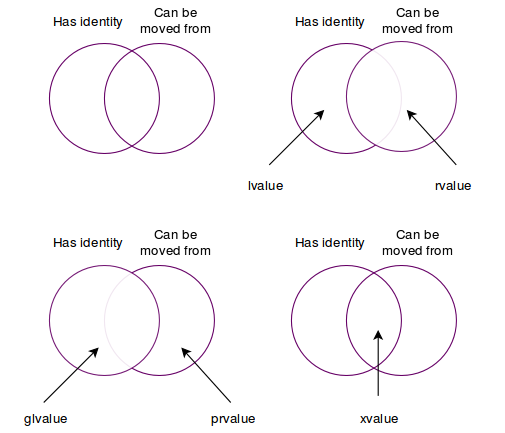
\includegraphics[height=.8\textheight]{valcat.png}

    \scalebox{.7}{(diagrams shamelessly stolen from \href{http://bajamircea.github.io/coding/cpp/2016/04/07/move-forward.html}{\texttt{bajamircea.github.io/coding/cpp/2016/04/07/move-forward.html}})}

\end{frame}

\begin{frame}[fragile]{Value categories with Venn diagrams}
    \begin{center}
        \scalebox{.7}{(diagrams shamelessly stolen from \href{http://bajamircea.github.io/coding/cpp/2016/04/07/move-forward.html}{\texttt{bajamircea.github.io/coding/cpp/2016/04/07/move-forward.html}})}
    \end{center}
    \begin{columns}
        \begin{column}{.7\textwidth}
            \begin{lstlisting}
struct S{ int x; };

S make_S(int x) {
    S s{.x = x};
    return s; // has no name after returning
}

int main() {
    S a = make_S(42); // `a` is an lvalue
                      // initialized with a prvalue

    S b = std::move(a); // prepare to die, `a`!
                        // now `a` became an xvalue

    auto x = a.x; // ERROR: `a` is in an undefined state
    a = make_S(13);
    x = a.x; // fine!
}
            \end{lstlisting}
        \end{column}
        \begin{column}{.25\textwidth}
            \only<1>{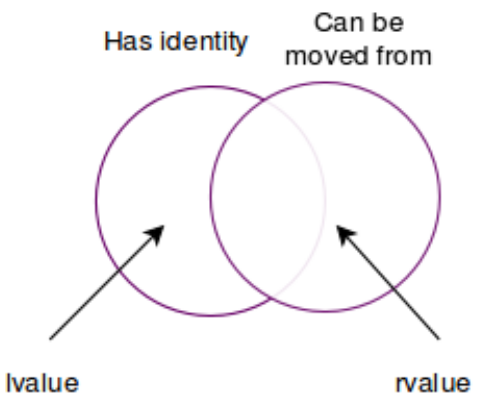
\includegraphics[width=\textwidth]{valcat1.png}}%
            \only<2>{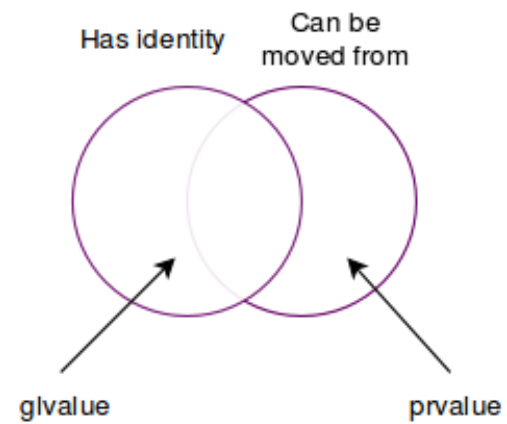
\includegraphics[width=\textwidth]{valcat2.png}}%
            \only<3>{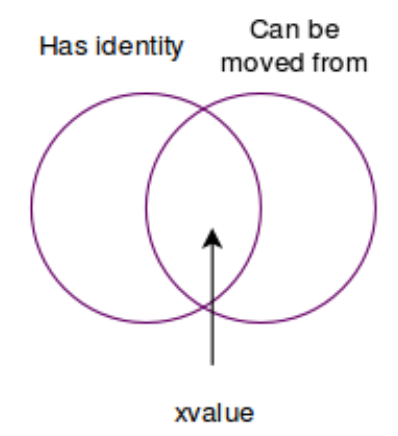
\includegraphics[width=\textwidth]{valcat3.png}}%
        \end{column}
    \end{columns}
\end{frame}

\begin{frame}[fragile]{Binding references to temporaries}
    \begin{center}
        \textbf{\textcolor{vertexDarkRed}{error:}} cannot bind non-const lvalue reference of type \enquote{\texttt{S*\&}} to an rvalue of type \enquote{\texttt{S*}}
    \end{center}
    \begin{columns}
        \begin{column}{.4\textwidth}
            \begin{lstlisting}
template <typename T>
void swap(T& a, T& b) { ... }

int main() {
    S a{1};
    S b{2};
    swap(&a, &b);
}
            \end{lstlisting}
        \end{column}
        \begin{column}{.55\textwidth}
            \begin{itemize}
                \item Memory addresses are always rvalues!
                \item One cannot refer to something that doesn't has a name\ldots
                \item \ldots except it is a const reference (lifetime extension)
            \end{itemize}
        \end{column}
    \end{columns}
\end{frame}

\begin{frame}[plain,noframenumbering]
    \centering
    \scalebox{3}{\texttt{std::move}}
\end{frame}

\begin{frame}[fragile]{\texttt{std::move}}
    \begin{columns}
        \begin{column}{.55\textwidth}
            \inputcpplisting{snippet31}
        \end{column}
        \begin{column}{.4\textwidth}
            \begin{itemize}
                \item \texttt{std::move} creates xvalues
                \item Syntax:
                \begin{itemize}
                    \item lvalue ref.: \texttt{S\&}
                    \item rvalue ref.: \texttt{S\&\&}
                \end{itemize}
            \end{itemize}
        \end{column}
    \end{columns}
\end{frame}

\begin{frame}[fragile]{Q: What is the output of the program?}
    \inputcpplisting{snippet33a}
\end{frame}

\begin{frame}[fragile]{A: \texttt{abac}}
    \begin{columns}
        \begin{column}{.5\textwidth}
            \inputcpplisting{snippet33a}
        \end{column}
        \begin{column}{.45\textwidth}
            \begin{itemize}
                \item \texttt{S s1}: no surprise
                \item \texttt{S s2(s1)}: no surprise
                \item \texttt{S s3(S\{\})}: \href{https://en.cppreference.com/w/cpp/language/copy_elision}{\textit{mandatory} copy elision (initializer is prvalue of the same class type})
                \item \texttt{S s4(std::move(s1))}: forced move construction
            \end{itemize}
        \end{column}
    \end{columns}
\end{frame}

\begin{frame}[fragile]{Q: What is the output of the program?}
    \inputcpplisting{snippet33b}
\end{frame}

% REMOVE_FOR_PRINT {
\addtocounter{framenumber}{-1}
\begin{frame}[fragile]{A: \texttt{a2a33}}
    \inputcpplisting{snippet33b}
\end{frame}
% REMOVE_FOR_PRINT }

\begin{frame}[fragile]{Q: What is the output of the program?}
    \inputcpplisting{snippet33c}
\end{frame}

\begin{frame}[fragile]{Q: What is the output of the program?}
    \begin{columns}
        \begin{column}{.46\textwidth}
            \inputcpplisting{snippet33c}
        \end{column}
        \begin{column}{.49\textwidth}
            \textbf{Compile-time error} (in all three cases)
            \begin{itemize}
                \item \texttt{f(s1)}: ambiguity between \texttt{2} and \texttt{1}
                \item \texttt{f(S\{\})}: ambiguity between \texttt{2} and \texttt{3}
                \item \texttt{f(std::move(s1)}: same as \texttt{f(S{})}
            \end{itemize}

            $\hookrightarrow$ compiler cannot differentiate between copy and reference overloads! (neither lvalue, nor rvalue)
        \end{column}
    \end{columns}
\end{frame}

\begin{frame}[fragile]{Q: What is the output of the program?}
    \inputcpplisting{snippet33d}
\end{frame}

\begin{frame}[fragile]{A: \texttt{23aa}}
    \begin{columns}
        \begin{column}{.46\textwidth}
            \inputcpplisting{snippet33d}
        \end{column}
        \begin{column}{.49\textwidth}
            \begin{itemize}
                \item \texttt{S\&\&}: object that nobody cares about anymore and which will die soon (cf. lifetime extension!)
                \item \texttt{std::move} does not actually kill, but makes the object look like a dying object
            \end{itemize}

            \begin{center}
                \begin{overpic}[width=.8\textwidth]{arya.png}
                    \put(10,10){\color{white}An rvalue has no name} 
                \end{overpic}
            \end{center}
        \end{column}
    \end{columns}

    {\footnotesize \textbf{NB:} an rvalue ref behaves like an lvalue ref except that it can bind to a temporary (an rvalue), whereas one cannot bind a (non const) lvalue ref to an rvalue.}
\end{frame}

\begin{frame}[fragile]{\texttt{std::move}}
    \begin{columns}
        \begin{column}{.55\textwidth}
            \inputcpplisting{snippet34}
        \end{column}
        \begin{column}{.4\textwidth}
            \textbf{So what does \texttt{std::move}?}
            \begin{itemize}
                \item does not \textit{move}
                \item does not destroy
                \item does nothing at all during runtime
                \item \textbf{unconditionally casts} its argument to an rvalue
            \end{itemize}
        \end{column}
    \end{columns}
\end{frame}

\begin{frame}[fragile]{Quick Bench: \href{http://quick-bench.com/7qTMMYSgUJG-lRg-B26ZX77vim0}{\texttt{tinyurl.com/y67sg7to}}}
    \begin{lstlisting}
std::vector<int> x(1000, 42);
std::vector<int> y(1000, 42);
for (auto _ : state) {
    auto tmp = x;
    x = y;
    y = tmp;
    benchmark::DoNotOptimize(x[345] + y[678]);
}
    \end{lstlisting}

    \begin{lstlisting}
std::vector<int> x(1000, 42);
std::vector<int> y(1000, 42);
for (auto _ : state) {
    auto tmp = std::move(x);
    x = std::move(y);
    y = std::move(tmp);
    benchmark::DoNotOptimize(x[345] + y[678]);
}
    \end{lstlisting}
\end{frame}

\begin{frame}{Quick Bench: \href{http://quick-bench.com/7qTMMYSgUJG-lRg-B26ZX77vim0}{\texttt{tinyurl.com/y67sg7to}}}
    \centering

    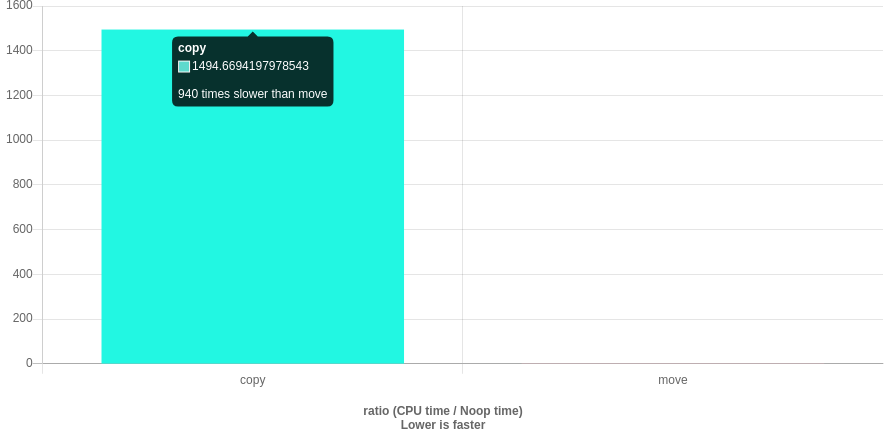
\includegraphics[height=.8\textheight]{benchmark_vec_mv.png}
\end{frame}

\begin{frame}[plain,noframenumbering]
    \centering
    \scalebox{3}{Universal References}
\end{frame}

\section{Universal References}

\begin{frame}[fragile]{Rvalue ref. or no rvalue ref.?}
    Rvalue refs are declared using \enquote{\&\&}: reasonable to assume that the presence of \enquote{\&\&} in a type declaration indicates an rvalue reference?
% REMOVE_FOR_PRINT {
    \only<2>{\textbf{No!}}
% REMOVE_FOR_PRINT }
    \begin{columns}
        \begin{column}{.45\textwidth}
            \begin{lstlisting}[numbers=none]
struct S{};

S&& s = S{};                // (1)

auto&& s2 = s;              // (2)

void f(S&& s);              // (3)

template <typename T>
void f(T&& t);              // (4)

template <typename T>
void f(const T&& t);        // (5)

template <typename T>
void f(std::vector<T>&& v); // (6)
            \end{lstlisting}
        \end{column}
        \begin{column}{.5\textwidth}
            \textbf{Does \enquote{\texttt{\&\&}} mean rvalue reference?}
            \begin{itemize}
                \item \texttt{(1)}: \only<1>{???}
% REMOVE_FOR_PRINT {
                \only<2>{yes}
% REMOVE_FOR_PRINT }
                \item \texttt{(2)}: \only<1>{???}
% REMOVE_FOR_PRINT {
                \only<2>{no}
% REMOVE_FOR_PRINT }
                \item \texttt{(3)}: \only<1>{???}
% REMOVE_FOR_PRINT {
                \only<2>{yes}
% REMOVE_FOR_PRINT }
                \item \texttt{(4)}: \only<1>{???}
% REMOVE_FOR_PRINT {
                \only<2>{no}
% REMOVE_FOR_PRINT }
                \item \texttt{(5)}: \only<1>{???}
% REMOVE_FOR_PRINT {
                \only<2>{yes${}^{\color{vertexDarkRed}\star}$}
% REMOVE_FOR_PRINT }
                \item \texttt{(6)}: \only<1>{???}
% REMOVE_FOR_PRINT {
                \only<2>{yes}
% REMOVE_FOR_PRINT }
            \end{itemize}
        \end{column}
    \end{columns}

    \only<2>{\footnotesize ${}^{\color{vertexDarkRed}\star}$ albeit questionable: \texttt{move} changes object in most cases $\not\leftrightarrow$ \texttt{const}}
\end{frame}

\addtocounter{framenumber}{-1}
\begin{frame}[plain,fragile]
    ${}^{\color{vertexDarkRed}\star}$ albeit questionable: \texttt{move} changes object in most cases $\not\leftrightarrow$ \texttt{const}

    \inputcpplisting{snippet42}
    
    \hfill \scalebox{1.5}{\ldots prints \texttt{A}}

    \begin{center}
        (cf. \href{https://stackoverflow.com/a/28595415}{\texttt{https://stackoverflow.com/a/28595415}})
    \end{center}
\end{frame}

\begin{frame}[fragile]{Universal references}
    \begin{columns}
        \begin{column}{.5\textwidth}
            \textbf{Universal references${}^{\color{vertexDarkRed}\dagger}$}
            \begin{itemize}
                \item Syntax (\texttt{x} is a universal reference):
                \begin{itemize}
                    \item \texttt{auto\&\& x}
                    \item \texttt{template <typename T>} \texttt{f(T\&\& x\ldots}
                \end{itemize}
                \item Rule of thumb: substitute fully qualified type into \texttt{auto} or \texttt{T} and reduce:
                \begin{itemize}
                    \item \texttt{\&\&} $\mapsto$ \texttt{\&\&} 
                    \item \texttt{\&\&\&} $\mapsto$ \texttt{\&} 
                    \item \texttt{\&\&\&\&} $\mapsto$ \texttt{\&\&} 
                \end{itemize}
            \end{itemize}
        \end{column}
        \begin{column}{.45\textwidth}
            \begin{lstlisting}[numbers=none]
std::vector<S> v;
auto&& s = v[0]; // S&&& -> S&

auto&& s2 = S{}; // S&&&& -> S&&
auto&& s3 = s2;  // S&&&  -> S&

// S&&&& -> S&&
auto&& s3 = std::move(s2);
            \end{lstlisting}
        \end{column}
    \end{columns}

    \vspace{5mm}

    \footnotesize ${}^{\color{vertexDarkRed}\dagger}$ \textit{Universal reference}: term introduced by Scott Meyers
\end{frame}

\begin{frame}[fragile]{Q: What is the output of the program?}
    \inputcpplisting{snippet35a}
\end{frame}

% REMOVE_FOR_PRINT {
\addtocounter{framenumber}{-1}
\begin{frame}[fragile]{A: \texttt{abb}}
    \inputcpplisting{snippet35a}

    \hfill \ldots how to preserve the value category?
\end{frame}
% REMOVE_FOR_PRINT }

\begin{frame}[fragile]{Q: What is the output of the program?}
    \inputcpplisting{snippet37}
\end{frame}

% REMOVE_FOR_PRINT {
\addtocounter{framenumber}{-1}
\begin{frame}[fragile]{A: \texttt{aba}}
    \inputcpplisting{snippet37}
\end{frame}
% REMOVE_FOR_PRINT }

\begin{frame}[fragile]{Q: What is the output of the program?}
    \inputcpplisting{snippet38}
\end{frame}

% REMOVE_FOR_PRINT {
\addtocounter{framenumber}{-1}
\begin{frame}[fragile]{A: \texttt{abaa}}
    \inputcpplisting{snippet38}
\end{frame}
% REMOVE_FOR_PRINT }

\begin{frame}[fragile]{Perfect forwarding}
    \centering
    \scalebox{1.5}{How do we fuse these implementations?}

    \begin{lstlisting}
// if `t` is an lvalue of type `S`
S& forward(S& t) {
    return t;
}

// if `t` is an rvalue of type `S`
S&& forward(S& t) { // not `S&&`!
    return std::move(t); // static_cast<S&&>(t)
}
    \end{lstlisting}

    \inputcpplisting{snippet36}
\end{frame}

\begin{frame}[fragile]{Q: What is the output of the program?}
    \inputcpplisting{snippet35b}
\end{frame}

\begin{frame}[fragile]{A: \texttt{abc}}
    \inputcpplisting{snippet35b}
    \textbf{Rule of thumb:} Use \texttt{std::move} for rvalues and \texttt{std::forward} for universal references
\end{frame}

\begin{frame}[fragile]{Q: Why can't we use perfect forwarding here?}
    \inputcpplisting{snippet9}

% REMOVE_FOR_PRINT {
    \only<2>{\textbf{A:} The first call in the loop might \textit{steal} the values, leading to unexpected behavior calling \texttt{op} in subsequent iterations.}
% REMOVE_FOR_PRINT }
\end{frame}

\begin{frame}[plain,noframenumbering]
    \centering
    \scalebox{3}{Reading x86-64 Assembly}

    \scalebox{2}{\ldots for fun and profit}
\end{frame}

\section{Reading Assembly for Fun and Profit}

\begin{frame}[fragile]{Function Prologue \& Epilogue}
    \begin{itemize}
        \item Few lines of code at the beginning (\textit{prologue}) and end (\textit{epilogue}) of a function, which \textbf{prepares} (and eventually restores)
        \begin{itemize}
            \item the \textbf{stack} and 
            \item \textbf{registers}
        \end{itemize}
        \item Not part of assembly: \textbf{convention} (defined \& interpreted differently by different OS and compilers)
    \end{itemize}

    \begin{columns}[t]
        \begin{column}{.45\textwidth}
            \textbf{Prologue}
            \begin{lstlisting}[language={}]
push rbp     ; rbp: frame pointer
mov rbp, rsp ; rsp: stack pointer
sub rsp, N
            \end{lstlisting}
            alternatively
            \begin{lstlisting}[language={}]
enter N, 0
            \end{lstlisting}
            (reserve \texttt{N} bytes on stack for local use)
        \end{column}
        \begin{column}{.45\textwidth}
            \textbf{Epilogue}
            \begin{lstlisting}[language={}]
mov rsp, rbp
pop rbp
ret
            \end{lstlisting}
            alternatively
            \begin{lstlisting}[language={}]
leave
ret
            \end{lstlisting}
        \end{column}
    \end{columns}
\end{frame}

\begin{frame}[fragile]{Stack frame for function call}
    \begin{columns}
        \begin{column}{.4\textwidth}
            \begin{itemize}
                \item \texttt{CALL} = \texttt{PUSH} \textit{address of next instruction} + \texttt{JMP} \textit{target}
                \item \texttt{RET} pops return address and transfers control there
                \item pass arguments 1 \ldots 6 in registers (\texttt{rsi}, \texttt{rdx}, \ldots)
            \end{itemize}
        \end{column}
        \begin{column}{.6\textwidth}
            \begin{Verbatim}
┌──────────────┐
│ ...          │
│ 8th Argument │ (rbp + 24)
│ 7th Argument │ (rbp + 16)
├──────────────┤
│ rip          │ (return address)
│ rbp          │ (rbp)
├──────────────┤
│ rbx          │
│ r12          │
│ r13          │ (rsp)
└──────────────┘
            \end{Verbatim}
            (stack frame for function call with 8 arguments and local registers \texttt{rbx}, \texttt{r12} and \texttt{r13})
        \end{column}
    \end{columns}
\end{frame}

\begin{frame}[fragile]{\texttt{lea} vs. \texttt{mov}}
    \begin{columns}
        \begin{column}{.5\textwidth}
            \begin{itemize}
                \item \texttt{lea}: \underline{l}oad \underline{e}ffective \underline{a}ddress
                \item puts memory address from \texttt{src} into the destination \texttt{dest}
                \item Example: \texttt{lea eax, [ebx+8]}
                \begin{itemize}
                    \item put \texttt{[ebx+8]} into \texttt{eax}
                    \item value of \texttt{eax} after instruction: \texttt{0x00403A48}
                \end{itemize}
                \item \ldots whereas: \texttt{mov eax, [ebx+8]}
                \begin{itemize}
                    \item value of \texttt{eax} after instruction: \texttt{0x0012C140}
                \end{itemize}
            \end{itemize}
        \end{column}
        \begin{column}{.5\textwidth}
            \begin{Verbatim}
           ┌──────────────────┐
           │ Registers        │
           ├──────────────────┤
           │ EAX = 0x00000000 │ 
           │ EBX = 0x00403A40 │ 
           └──────────────────┘
           ┌────────────┐
           │ Memory     │
           ├────────────┤
0x00403A40 │ 0x7C81776F │ 
0x00403A44 │ 0x7C911000 │ 
0x00403A48 │ 0x0012C140 │ 
0x00403A4C │ 0x7FFDB000 │ 
           └────────────┘
            \end{Verbatim}
        \end{column}
    \end{columns}
\end{frame}

\begin{frame}[fragile]{Reading assembly for fun and profit}
    \begin{columns}[t]
        \begin{column}{.45\textwidth}
            \inputcpplisting{snippet5a}
            
            \only<2>{%
            \inputasmlisting{snippet5b}}
        \end{column}
        \begin{column}{.45\textwidth}
            \inputasmlisting{snippet5a}
        \end{column}
    \end{columns}
\end{frame}

\begin{frame}[fragile]{Reading assembly for fun and profit}
    \begin{columns}[t]
        \begin{column}{.45\textwidth}
            \inputcpplisting{snippet6a}

            \only<2>{%
            \inputasmlisting{snippet6b}}
        \end{column}
        \begin{column}{.45\textwidth}
            \inputasmlisting{snippet6a}
        \end{column}
    \end{columns}

\end{frame}

\begin{frame}[fragile]{Reading assembly for fun and profit}
    \begin{columns}[t]
        \begin{column}{.45\textwidth}
            \inputcpplisting{snippet1a}
        \end{column}
        \begin{column}{.45\textwidth}
            \inputasmlisting{snippet1a}
        \end{column}
    \end{columns}
\end{frame}


\section{Implicit Costs of \texttt{const\&}}

\begin{frame}[fragile]{Implicit Costs of using \texttt{const\&}}
    \begin{columns}[t]
        \begin{column}{.45\textwidth}
            \inputcpplisting{snippet1a}
        \end{column}
        \begin{column}{.45\textwidth}
            \inputcpplisting{snippet2a}
        \end{column}
    \end{columns}
\end{frame}

\begin{frame}[fragile]{Implicit Costs of using \texttt{const\&}}
    \begin{columns}[t]
        \begin{column}{.45\textwidth}
            \inputasmlisting{snippet1a}
        \end{column}
        \begin{column}{.45\textwidth}
            \inputasmlisting{snippet2a}
        \end{column}
    \end{columns}
\end{frame}

\begin{frame}[fragile]{Implicit Costs of using \texttt{const\&}}
    \begin{columns}[t]
        \begin{column}{.45\textwidth}
            \inputasmlisting{snippet1b}

            \footnotesize
            \only<1>{\textbf{NB \#1:} adjusting \texttt{rsp} in function prologue necessary when function is not a leaf function since callee have to know where to start saving variables on stack. (Adjusting \texttt{rsp} can be ommitted in leaf functions.)}
            \only<2>{\textbf{NB \#2:} Offset \texttt{x} in \texttt{sub rsp, x} is objective of optimizations such as alignment: ABI requires stack to be aligned to 16 bytes.}
        \end{column}
        \begin{column}{.45\textwidth}
            \inputasmlisting{snippet2b}
        \end{column}
    \end{columns}
\end{frame}

\begin{frame}[fragile]{Implicit Costs of using \texttt{const\&}}
    \begin{columns}[t]
        \begin{column}{.45\textwidth}
            \inputasmlisting{snippet1b}

            \footnotesize
            \only<1>{\textbf{NB \#1:} adjusting \texttt{rsp} in function prologue necessary when function is not a leaf function since callee have to know where to start saving variables on stack. (Adjusting \texttt{rsp} can be ommitted in leaf functions.)}
            \only<2>{\textbf{NB \#2:} Offset \texttt{x} in \texttt{sub rsp, x} is objective of optimizations such as alignment: ABI requires stack to be aligned to 16 bytes.}
        \end{column}
        \begin{column}{.45\textwidth}
            \inputasmlisting{snippet2b}
        \end{column}
    \end{columns}
\end{frame}

\begin{frame}[fragile]{Implicit Costs of using \texttt{const\&}}
    \begin{columns}[t]
        \begin{column}{.45\textwidth}
            \inputcpplisting{snippet43a}
        \end{column}
        \begin{column}{.5\textwidth}
            \inputasmlisting{snippet43a}
        \end{column}
    \end{columns}
    \only<1>{%
    Even though we \textit{only} pass a reference, we pay the cost of the complex object \texttt{std::string} (i.e., first bit is tested for short string optimization)

    \begin{center}
        \scalebox{1.2}{$\hookrightarrow$ prefer views such as \texttt{std::string\_view} or \texttt{std::span}}
    \end{center}}
    \only<2>{${}^{\color{vertexDarkRed}\star}$Confession: switching to \texttt{libstdc++} resolves this issue here}
\end{frame}

\begin{frame}[fragile]{Will it compile?}
    \begin{columns}
        \begin{column}{.45\textwidth}
            \inputcpplisting{snippet39}
        \end{column}
        \begin{column}{.45\textwidth}
            \only<2>{%
            \textbf{\textcolor{vertexDarkRed}{No!}}
            \begin{itemize}
                \item Constructor takes by reference
                \item References to automatic storage objects are not constant expressions!
                \item Solutions?
            \end{itemize}}
        \end{column}
    \end{columns}

    \vspace{1cm}

    \begin{lstlisting}
template <std::size_t N>
constexpr span(const std::array<value_type, N>& arr) noexcept;
    \end{lstlisting}
    \href{https://en.cppreference.com/w/cpp/container/span/span}{\texttt{cppreference.com/w/cpp/container/span/span}}
\end{frame}

\begin{frame}[fragile]{Will it compile?}
    \inputcpplisting{snippet40}
\end{frame}

\begin{frame}[fragile]{Nota bene \ldots}
    this will work though, since reference / pointer does not \textit{escape} constant expression \ldots
    \inputcpplisting{snippet41}
\end{frame}

\begin{frame}[plain,noframenumbering]
    \centering
    \scalebox{3}{Time to grab some covfefe}

    \vspace{1cm}

    
\includegraphics[width=.3\textwidth]{trump}
\end{frame}

\addtocounter{framenumber}{-1}
\begin{frame}[fragile]{A Short Quiz for the Break}
    \begin{lstlisting}[language=python]
#!/usr/bin/env python3

def f(x):
    if x + 1 is 1 + x:
        return False
    if x + 2 is not 2 + x:
        return False

    return True
    \end{lstlisting}

    Find all \texttt{x} for which \texttt{f(x)} returns \texttt{True} !
\end{frame}

\addtocounter{framenumber}{-1}
\begin{frame}[fragile]{A Short Quiz for the Break}
    \begin{lstlisting}[language=python]
#!/usr/bin/env python3

def f(x):
    if x + 1 is 1 + x:
        return False
    if x + 2 is not 2 + x:
        return False

    return True
    \end{lstlisting}

    Find all \texttt{x} for which \texttt{f(x)} returns \texttt{True} !

    \begin{center}
        \scalebox{1.5}{Answer: \texttt{f(x=-7)}}
    \end{center}
\end{frame}

\begin{frame}[plain,noframenumbering]
    \centering
    \scalebox{3}{Dangling References}
\end{frame}

\section{Dangling references}

\begin{frame}[fragile]{Will it compile?}
    \inputcpplisting{snippet22a}

    \only<2>{\textbf{\textcolor{vertexDarkRed}{error:}} cannot bind non-const lvalue reference of type \enquote{S\&} to an rvalue of type \enquote{S}}%
\end{frame}

\begin{frame}[fragile]{Will it invoke undefined behavior?}
    \inputcpplisting{snippet22b}

    \hfill \ldots binding a reference to a temporary???
\end{frame}

\begin{frame}[fragile]{Temporary object lifetime extension}
    \inputcpplisting{snippet22b}

    \href{https://en.cppreference.com/w/cpp/language/lifetime}{\texttt{cppreference.com}: \enquote{The lifetime of a temporary object may be extended by binding to a const lvalue reference or to an rvalue reference (since C++11).}}
\end{frame}

\begin{frame}[fragile]{Q: What is the output of the program?}
    \inputcpplisting{snippet29}
\end{frame}

\begin{frame}[fragile]{A: \texttt{a1b1a2xb2}}
    \begin{columns}
        \begin{column}{.55\textwidth}
            \inputcpplisting{snippet29}
        \end{column}
        \begin{column}{.4\textwidth}
            \textbf{Dangling reference!!!}
            \begin{itemize}
                \item lifetime extension only for result of the temporary expression, \textbf{not any sub-expression}
                \item use \href{https://clang.llvm.org/docs/AddressSanitizer.html}{address sanitizer}!    
            \end{itemize}
        \end{column}
    \end{columns}
\end{frame}

\begin{frame}[plain,noframenumbering]
    \centering
    \scalebox{2.}{contrived?}
\end{frame}

\begin{frame}[fragile]{Reference lifetime extension}
    \begin{center}
        \scalebox{.7}{(derived from \href{https://abseil.io/tips/107}{\texttt{abseil.io}: Tip of the Week \#107: \enquote{Reference Lifetime Extension})}}
    \end{center}

    \begin{lstlisting}
std::vector<std::string_view> explode(const std::string& s);

for (std::string_view s: explode(str_cat("oo", "ps"))) { // WRONG!
    [...]
    \end{lstlisting}
\end{frame}

\begin{frame}[fragile]{Q: What is the output of the program?}
    \begin{columns}
        \begin{column}{.45\textwidth}
            \inputcpplisting{snippet30}
        \end{column}
        \begin{column}{.5\textwidth}
            \only<2>{%
            \textbf{Dangling reference!!!}
            \begin{itemize}
                \item \texttt{std::vector} needs to reallocate all the space the second time an element is pushed 
                \item use \href{https://clang.llvm.org/docs/AddressSanitizer.html}{address sanitizer}!    
            \end{itemize}}
        \end{column}
    \end{columns}
\end{frame}

\begin{frame}[plain,noframenumbering]
    \centering
    \scalebox{3}{\texttt{std::move} in the wild}
\end{frame}

\section{\texttt{std::move} in the wild}

\begin{frame}[fragile]{Moving \texttt{std::string}}
    \centering
    \scalebox{.7}{(derived from \href{https://youtu.be/oTMSgI1XjF8}{CppCon 2019: \textit{Ben Deane} \enquote{Everyday Efficiency: In-Place Construction (Back to Basics?)})}}

    \begin{lstlisting}
static void cp_small_str(benchmark::State& state) {
    for (auto _ : state) {
        std::string original("small");
        benchmark::DoNotOptimize(original);
        std::string copied = original;
        benchmark::DoNotOptimize(copied);
    }
}
BENCHMARK(cp_small_str);
    \end{lstlisting}

    \begin{lstlisting}
static void mv_small_str(benchmark::State& state) {
    for (auto _ : state) {
        std::string original("small");
        benchmark::DoNotOptimize(original);
        std::string moved = std::move(original);
        benchmark::DoNotOptimize(moved);
    }
}
BENCHMARK(mv_small_str);
    \end{lstlisting}
\end{frame}

\begin{frame}[fragile]{Moving \texttt{std::string}}
    \centering
    \scalebox{.7}{(derived from \href{https://youtu.be/oTMSgI1XjF8}{CppCon 2019: \textit{Ben Deane} \enquote{Everyday Efficiency: In-Place Construction (Back to Basics?)})}}

    \begin{lstlisting}
static void cp_long_str(benchmark::State& state) {
    for (auto _ : state) {
        std::string original("this is too long for short string optimization");
        benchmark::DoNotOptimize(original);
        std::string copied = original;
        benchmark::DoNotOptimize(copied);
    }
}
BENCHMARK(cp_long_str);
    \end{lstlisting}

    \begin{lstlisting}
static void mv_long_str(benchmark::State& state) {
    for (auto _ : state) {
        std::string original("this is too long for short string optimization");
        benchmark::DoNotOptimize(original);
        std::string moved = std::move(original);
        benchmark::DoNotOptimize(moved);
    }
}
BENCHMARK(mv_long_str);
    \end{lstlisting}
\end{frame}

\begin{frame}{Moving \texttt{std::string}}
    \centering
    \scalebox{1.5}{Quick Bench result}

    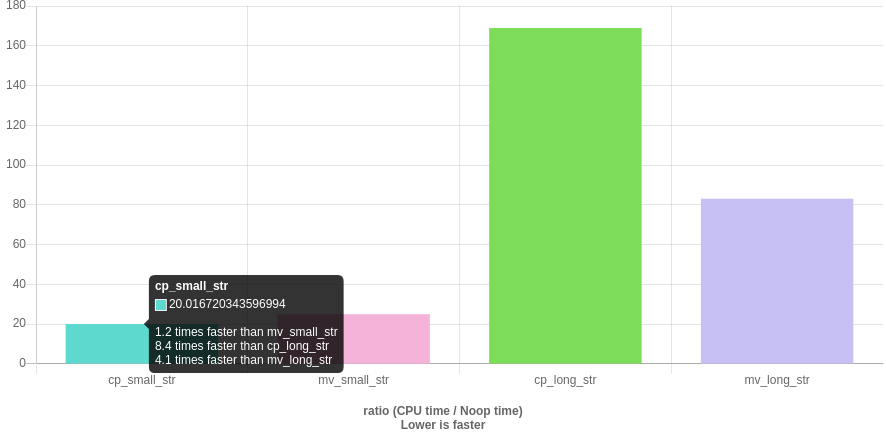
\includegraphics[width=.9\textwidth]{benchmark_str_cp_mv.png}

    Quick Bench: \href{http://quick-bench.com/l_4Ith4ZvZbSE0UIfIQXVpkg84A}{\texttt{tinyurl.com/yybmdngv}}
\end{frame}

\begin{frame}[fragile]{Moving \texttt{std::string}}
    \centering

    \begin{columns}[t]
        \begin{column}{.45\textwidth}
            \begin{block}{Copy small \texttt{std::string}}
                \begin{enumerate}
                    \item copy stack allocated data
                \end{enumerate}
            \end{block}
        \end{column}
        \begin{column}{.45\textwidth}
            \begin{block}{Move small \texttt{std::string}}
                \begin{enumerate}
                    \item copy stack allocated data
                    \item set string length of moved string to zero
                \end{enumerate}
            \end{block}
        \end{column}
    \end{columns}

    \vspace{5mm}

    \begin{center}
        \scalebox{1.5}{$\hookrightarrow$ moving is not necessarily better than copying!}
    \end{center}
\end{frame}

\begin{frame}[fragile]{Moving \texttt{std::map}}
    \textbf{Did they forget to mark the move ctor \texttt{noexcept}?} \only<2>{\textcolor{vertexDarkRed}{No!}}

    \begin{columns}[t]
        \begin{column}{.45\textwidth}
            \begin{lstlisting}[numbers=none]
// since C++11
std:map(const std:map&&)

// until C++17
std:map& operator(std:map&&)

// since C++17
std:map& operator(std:map&&) noexcept
            \end{lstlisting}
        \end{column}
        \begin{column}{.5\textwidth}
            \begin{itemize}
                \item<2> Move ctor needs to allocate new sentinel node, because moved from container must still be a valid container (albeit in an unspecified state)
                \item<2> Move assignment can swap, thus no need to allocate
            \end{itemize}
        \end{column}
    \end{columns}

    \only<2>{%
    \begin{center}
        \scalebox{1.5}{$\hookrightarrow$ move ctor of \texttt{std::map} allocates heap space!}

        \scalebox{.8}{(Billy O'Neal: \href{https://twitter.com/MalwareMinigun/status/1165310509022736384}{\texttt{twitter.com/MalwareMinigun/status/1165310509022736384})}}
    \end{center}}
\end{frame}

\begin{frame}[fragile]{Moving \texttt{std::map}}
    \begin{lstlisting}
static void rvo(benchmark::State& state) {
    for (auto _ : state) {
        auto m = []() -> std::map<int, int> {
            std::map<int, int> m{{0, 42}};
            return m;
        }();
        benchmark::DoNotOptimize(m);
    }
}
BENCHMARK(rvo);
    \end{lstlisting}

    \begin{lstlisting}
static void fmove(benchmark::State& state) {
    for (auto _ : state) {
        auto m = []() -> std::map<int, int> {
            std::map<int, int> m{{0, 42}};
            return std::move(m);
        }();
        benchmark::DoNotOptimize(m);
    }
}
BENCHMARK(fmove);
    \end{lstlisting}
\end{frame}
\begin{frame}[fragile]{Moving \texttt{std::map}}
    \begin{lstlisting}
static void copy(benchmark::State& state) {
    for (auto _ : state) {
        std::map<int, int> m{{0, 42}};
        benchmark::DoNotOptimize(m);
        auto m2 = m;
        benchmark::DoNotOptimize(m2);
    }
}
BENCHMARK(copy);
    \end{lstlisting}
\end{frame}

\begin{frame}{Moving \texttt{std::map}}
    \centering
    \scalebox{1.5}{Quick Bench result}

    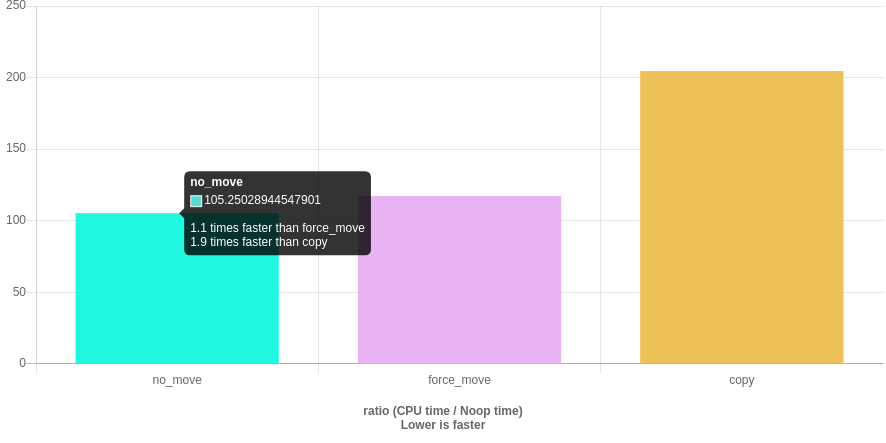
\includegraphics[width=.9\textwidth]{benchmark_map_mv.png}

    Quick Bench: \href{http://quick-bench.com/7L-__vxvraDDacztJoalrjBrMUA}{\texttt{tinyurl.com/y57egvjp}}
\end{frame}

\begin{frame}[plain,noframenumbering]
    \centering
    \scalebox{5}{Why?}
\end{frame}

\begin{frame}[fragile]{Does this code bother anyone?}
    \inputcpplisting{snippet3}
\end{frame}

\begin{frame}[plain,noframenumbering]
    \centering
    \scalebox{2}{Interlude}

    \scalebox{3}{What happens on \texttt{return}?}
\end{frame}

\section{What Happens on \texttt{return}?}

\begin{frame}[fragile]{Will it compile?}
    \inputcpplisting{snippet8}
\end{frame}

\begin{frame}[fragile]{Implicit conversion to the function return type}
    \inputcpplisting{snippet8}

    \textbf{\textcolor{vertexDarkRed}{error:}} could not convert \enquote{42} from \enquote{int} to \enquote{B}
\end{frame}

\begin{frame}[fragile]{Implicit conversion to the function return type}
    \begin{columns}
        \begin{column}{.55\textwidth}
            \textbf{Implicit conversion}
            \begin{itemize}
                \item \ldots if ctor is \textbf{not} marked \texttt{explicit}
                \item Examples: 
                \begin{itemize}
                    \item \href{https://en.cppreference.com/w/cpp/utility/optional/optional}{\texttt{std::optional(T\&\&)}}
                    \item \href{https://en.cppreference.com/w/cpp/string/basic_string/basic_string}{\texttt{std::string(const char*)}}
                \end{itemize}
            \end{itemize}
        \end{column}
        \begin{column}{.35\textwidth}
            \inputcpplisting{snippet27}
        \end{column}
    \end{columns}
\end{frame}

\begin{frame}[fragile]{Q: What is the output of the program?}
    \begin{center}
        Compiler flags: \texttt{-std=c++14 -fno-elide-constructors}
    \end{center}

    \inputcpplisting{snippet4a}
\end{frame}

\begin{frame}[fragile]{A: \texttt{ac}, \texttt{acc}, \texttt{acc}}
    \begin{center}
        Compiler flags: \texttt{-std=c++14 -fno-elide-constructors}
    \end{center}

    \inputcpplisting{snippet4a}
\end{frame}

\begin{frame}[fragile]{Q: What is the output of the program?}
    \begin{center}
        Compiler flags: \texttt{-std=c++17}
    \end{center}

    \inputcpplisting{snippet4b}
\end{frame}

\begin{frame}[fragile]{A: \texttt{a}, \texttt{a}, \texttt{a}}
    \begin{center}
        Compiler flags: \texttt{-std=c++17}
    \end{center}

    \inputcpplisting{snippet4b}
\end{frame}

\begin{frame}[plain,noframenumbering]
    \centering
    \scalebox{5}{\only<1>{Why?}\only<2>{RVO!}}

    \only<2>{Ben Deane: \enquote{Perhaps the most important optimization the compiler does}}
\end{frame}

\begin{frame}{Copy Elision}
    \begin{columns}
        \begin{column}{.45\textwidth}
            \inputcpplisting{snippet10}
        \end{column}
        \begin{column}{.5\textwidth}
            Mandatory elision of copy/move operations since \texttt{C++17}):
            \begin{itemize}
                \item Return statement: when operand is a \texttt{prvalue} of same class type as return type
                \item Initialization of a variable: when initializer expression is a \texttt{prvalue} of same class type as the variable type
            \end{itemize}
        \end{column}
    \end{columns}
    \ldots even if the copy/move constructor and the destructor have observable side-effects!
    \vspace{.5cm}

    \centering
    \scalebox{1.5}{\textbf{Rule of thumb: avoid naming return values}}
\end{frame}

\section{RVO in Depth}

\begin{frame}[plain,noframenumbering]
    \centering
    \scalebox{3}{RVO in Depth}
\end{frame}

\begin{frame}[fragile]{\texttt{C++} Objects in Assembly}
    \begin{columns}[t]
        \begin{column}{.45\textwidth}
            \inputcpplisting{snippet20}
        \end{column}
        \begin{column}{.45\textwidth}
            \begin{lstlisting}[language={},morekeywords={rdi},numbers=none]
  | main:
14|   push rbp
14|   mov rbp, rsp
14|   sub rsp, 16
14|   mov dword ptr [rbp - 4], 0
15|   lea rdi, [rbp - 16]
15|   mov esi, 1
15|   mov edx, 2
15|   mov ecx, 3
15|   call S::S(int, int, int)
16|   lea rdi, [rbp - 16]
16|   call S::sum()
16|   mov dword ptr [rbp - 4], eax
17|   lea rdi, [rbp - 16]
17|   call S::~S()
17|   mov eax, dword ptr [rbp - 4]
17|   add rsp, 16
17|   pop rbp
17|   ret
            \end{lstlisting}
        \end{column}
    \end{columns}
\end{frame}

\begin{frame}[fragile]{\texttt{C++} Objects in Assembly}
    \begin{columns}[t]
        \begin{column}{.45\textwidth}
            \inputcpplisting{snippet20}
        \end{column}
        \begin{column}{.45\textwidth}
            \begin{lstlisting}[language={},morekeywords={rdi},numbers=none]
  | S::S(int, int, int):
 5|   push rbp
 5|   mov rbp, rsp
 5|   mov qword ptr [rbp - 8], rdi
 5|   mov dword ptr [rbp - 12], esi
 5|   mov dword ptr [rbp - 16], edx
 5|   mov dword ptr [rbp - 20], ecx
 5|   mov rax, qword ptr [rbp - 8]
 5|   mov ecx, dword ptr [rbp - 12]
 5|   mov dword ptr [rax], ecx
 5|   mov ecx, dword ptr [rbp - 16]
 5|   mov dword ptr [rax + 4], ecx
 5|   mov ecx, dword ptr [rbp - 20]
 5|   mov dword ptr [rax + 8], ecx
 5|   pop rbp
 5|   ret
            \end{lstlisting}
        \end{column}
    \end{columns}
\end{frame}

\begin{frame}[fragile]{\texttt{C++} Objects in Assembly}
    \begin{columns}[t]
        \begin{column}{.45\textwidth}
            \inputcpplisting{snippet20}
        \end{column}
        \begin{column}{.45\textwidth}
            \begin{lstlisting}[language={},morekeywords={rdi},numbers=none]
  | S::sum():
 9|   push rbp
 9|   mov rbp, rsp
 9|   mov qword ptr [rbp - 8], rdi
 9|   mov rax, qword ptr [rbp - 8]
10|   mov ecx, dword ptr [rax]
10|   add ecx, dword ptr [rax + 4]
10|   add ecx, dword ptr [rax + 8]
10|   mov eax, ecx
10|   pop rbp
10|   ret
            \end{lstlisting}
        \end{column}
    \end{columns}
\end{frame}

\begin{frame}[fragile]{RVO in Assembly}
    \begin{columns}[t]
        \begin{column}{.45\textwidth}
            \inputcpplisting{snippet7}
        \end{column}
        \begin{column}{.45\textwidth}
            \begin{lstlisting}[language={},morekeywords={rdi},numbers=none]
# g92 -fno-elide-constructors
  | g():
  |   [...]
14|   lea rax, [rbp-20]
14|   mov rdi, rax
14|   call f()
14|   lea rdx, [rbp-20]
14|   lea rax, [rbp-24]
14|   mov rsi, rdx
14|   mov rdi, rax
14|   call S::S(S&&)
14|   lea rax, [rbp-20]
14|   mov rdi, rax
14|   call S::~S()
15|   mov ebx, DWORD PTR [rbp-24]
14|   lea rax, [rbp-24]
14|   mov rdi, rax
14|   call S::~S()
15|   mov eax, ebx
  |   [...]      
            \end{lstlisting}
        \end{column}
    \end{columns}
\end{frame}

\begin{frame}[fragile]{RVO in Assembly}
    \begin{columns}[t]
        \begin{column}{.45\textwidth}
            \inputcpplisting{snippet7}
        \end{column}
        \begin{column}{.45\textwidth}
            \begin{lstlisting}[language={},morekeywords={rdi},numbers=none]
# g92 -fno-elide-constructors
  | f():
  |   [...]
 9|   mov QWORD PTR [rbp-24], rdi
10|   lea rax, [rbp-4]
10|   mov esi, 42
10|   mov rdi, rax
10|   call S::S(int)
10|   lea rdx, [rbp-4]
10|   mov rax, QWORD PTR [rbp-24]
10|   mov rsi, rdx
10|   mov rdi, rax
10|   call S::S(S&&)
10|   lea rax, [rbp-4]
10|   mov rdi, rax
10|   call S::~S()
  |   [...]      
            \end{lstlisting}
        \end{column}
    \end{columns}
\end{frame}

\begin{frame}[fragile]{RVO in Assembly}
    \begin{columns}[t]
        \begin{column}{.45\textwidth}
            \begin{lstlisting}[language={},morekeywords={rdi}]
# g92 -fno-elide-constructors
f():
  [...]
  mov QWORD PTR [rbp-24], rdi
  lea rax, [rbp-4]
  mov esi, 42
  mov rdi, rax
  call S::S(int)
  lea rdx, [rbp-4]
  mov rax, QWORD PTR [rbp-24]
  mov rsi, rdx
  mov rdi, rax
  call S::S(S&&)
  lea rax, [rbp-4]
  mov rdi, rax
  call S::~S()
  nop
  mov rax, QWORD PTR [rbp-24]
  leave
  ret
            \end{lstlisting}
        \end{column}
        \begin{column}{.45\textwidth}
            \begin{lstlisting}[language={},morekeywords={rdi}]
# g92
f():
  [...]
  mov QWORD PTR [rbp-8], rdi
  mov rax, QWORD PTR [rbp-8]
  mov esi, 42
  mov rdi, rax
  call S::S(int)
  mov rax, QWORD PTR [rbp-8]
  leave
  ret
            \end{lstlisting}
        \end{column}
    \end{columns}
\end{frame}

\begin{frame}[fragile]{RVO in Assembly}
    \begin{columns}[t]
        \begin{column}{.45\textwidth}
            \begin{lstlisting}[language={},morekeywords={rdi}]
# g92 -fno-elide-constructors
g():
  [...]
  lea rax, [rbp-20]
  mov rdi, rax
  call f()
  lea rdx, [rbp-20]
  lea rax, [rbp-24]
  mov rsi, rdx
  mov rdi, rax
  call S::S(S&&)
  lea rax, [rbp-20]
  mov rdi, rax
  call S::~S()
  mov ebx, DWORD PTR [rbp-24]
  lea rax, [rbp-24]
  mov rdi, rax
  call S::~S()
  mov eax, ebx
  [...]      
            \end{lstlisting}
        \end{column}
        \begin{column}{.45\textwidth}
            \begin{lstlisting}[language={},morekeywords={rdi}]
# g92
g():
  [...]
  lea rax, [rbp-20]
  mov rdi, rax
  call f()
  mov ebx, DWORD PTR [rbp-20]
  lea rax, [rbp-20]
  mov rdi, rax
  call S::~S()
  mov eax, ebx
            \end{lstlisting}
        \end{column}
    \end{columns}
\end{frame}

\begin{frame}[fragile]{(N)RVO or no (N)RVO?}
    \inputcpplisting{snippet21}
    \begin{itemize}
        \item \texttt{f1}: \only<1>{???}\only<2>{RVO}
        \item \texttt{f2}: \only<1>{???}\only<2>{\texttt{call S::S(S\&\&)}}
        \item \texttt{f3}: \only<1>{???}\only<2>{RVO}
        \item \texttt{f4}: \only<1>{???}\only<2>{\texttt{call S::S(const S\&)} (silently revert to a copy!)}
    \end{itemize}
\end{frame}

\begin{frame}[fragile]{(N)RVO or no (N)RVO?}
    \inputcpplisting{snippet25}
    \begin{itemize}
        \item \texttt{f1}: \only<1>{???}\only<2>{No RVO: the object has to be constructed inside the function}
        \item \texttt{f2}: \only<1>{???}\only<2>{same as \texttt{f1}}
        \item \texttt{f3}: \only<1>{???}\only<2>{same as \texttt{f1}}
    \end{itemize}
\end{frame}

\begin{frame}[fragile]{(N)RVO or no (N)RVO?}
    \inputcpplisting{snippet23}

    \only<2>{No RVO: \texttt{call S::S(S const\&)}}
\end{frame}

\begin{frame}[fragile]{(N)RVO or no (N)RVO?}
    \inputcpplisting{snippet26}
    \begin{itemize}
        \item \texttt{f1}: \only<1>{???}\only<2>{RVO: type of ternary is prvalue}
        \item \texttt{f2}: \only<1>{???}\only<2>{No RVO: type of ternary is lvalue reference}
    \end{itemize}

\end{frame}

\begin{frame}[fragile]{(N)RVO or no (N)RVO?}
    \inputcpplisting{snippet24}
    \begin{itemize}
        \item \texttt{g1}: \only<1>{???}\only<2>{no RVO: \texttt{call S::S(S\&\&)}}
        \item \texttt{g2}: \only<1>{???}\only<2>{same as \texttt{g1}}
        \item \texttt{g3}: \only<1>{???}\only<2>{no RVO: \texttt{call S::S(const S\&)}}
        \item \texttt{g4}: \only<1>{???}\only<2>{same as \texttt{g3}}
    \end{itemize}
\end{frame}

\begin{frame}[fragile]{(N)RVO or no (N)RVO?}
    \begin{center}
        \scalebox{.7}{(derived from \href{https://youtu.be/ZxWjii99yao}{CppCon 2019: \textit{Jason Turner} \enquote{Great C++ is\_trivial}})}
    \end{center}

    \textbf{No (N)RVO in any of these examples!}
    \begin{lstlisting}
S g1() { auto [s1, s2] = f(); return s1; } // copy
S g2() { auto&& [s1, s2] = f(); return s1; } // copy: no implicit move yet (?)
S g3() { auto [s1, s2] = f(); return std::move(s1); } // move
S g4() { auto&& [s1, s2] = f(); return std::move(s1); } // move
    \end{lstlisting}
    
    \hfill \ldots \texttt{return std::move} is not always bad

    \textbf{Why?} Structured bindings:
    \begin{itemize}
        \item Creation of temporary object \texttt{e}
        \item Like a reference: structured binding is an alias into \texttt{e}
    \end{itemize}
\end{frame}

\begin{frame}{Implicit move}
    \begin{center}
        \scalebox{1.5}{\texttt{return std::move} is not yet necessarily a code smell}

        (use \texttt{-Wpessimizing-move})
    \end{center}

    \href{https://en.cppreference.com/w/cpp/language/return}{\textbf{Automatic move from local variables and parameters \underline{if}:}}
    \begin{itemize}
        \item return expression names a variable whose type is either
        \begin{itemize}
            \item an object type or (since \texttt{C++11})
            \item a rvalue reference to object type (since \texttt{C++20}${}^{\textcolor{vertexDarkRed}\star}$)
        \end{itemize}
        \item \ldots and that variable is declared
        \begin{itemize}
            \item in the body or
            \item as a parameter of
        \end{itemize}
        \item \ldots the innermost enclosing function or lambda expression
    \end{itemize}

    ${}^{\textcolor{vertexDarkRed}\star}$ \scalebox{.8}{\href{http://www.open-std.org/jtc1/sc22/wg21/docs/papers/2019/p1825r0.html}{\texttt{P1825R0}} (not yet implemented in GCC or Clang: \href{https://en.cppreference.com/w/cpp/compiler_support}{cppreference.com/w/cpp/compiler\_support})}
\end{frame}

\begin{frame}[fragile]{Q: Why can't we use perfect forwarding here?}
    \inputcpplisting{snippet9}

    \only<2>{\textbf{A:} The first call in the loop might \textit{steal} the values, leading to unexpected behavior calling \texttt{op} in subsequent iterations.}
\end{frame}

\begin{frame}[plain,noframenumbering]
    \centering
    \scalebox{3}{Perfect Backwarding}
\end{frame}

\section{Perfect Backwarding}

\begin{frame}[fragile]{Forwarding Values and Preserving Value Category}
    \centering

    \scalebox{.7}{(derived from \href{https://youtu.be/hwT8K3-NH1w}{CppCon 2018: \textit{Hayun Ezra Chung} \enquote{Forwarding Values... and Backwarding Them Too?})}}

    \only<1>{\inputcpplisting{snippet11a}}%
    \only<2>{\inputcpplisting{snippet11b}}%
    \only<3>{\inputcpplisting{snippet11c}}%
\end{frame}

\begin{frame}[fragile]{Backwarding Values and Preserving Value Category}
    \only<1>{\inputcpplisting{snippet18a}}%
    \only<2>{\inputcpplisting{snippet18b}}%
\end{frame}

\begin{frame}[fragile]{Backwarding Values and Preserving Value Category}
    \textbf{Q:} Why is this a bad idea?
    \begin{lstlisting}
auto&& visit(auto visitor) {
    auto&& result = visitor(resource);
    return result;
}
    \end{lstlisting}
    
    \only<2>{%
    \textbf{A:} Dangling reference for

    \centering
    \texttt{visit([](Resource \&r) -> Resource \{ return r; \}));}

    \vspace{.5cm}

    \begin{center}
        \scalebox{1.5}{\texttt{auto\&\&} is always a reference!}
    \end{center}}
\end{frame}

\begin{frame}[fragile]{Backwarding Values and Preserving Value Category}
    \only<1>{\inputcpplisting{snippet12a}}%
    \only<2>{\inputcpplisting{snippet12b}}
\end{frame}

\begin{frame}[fragile]{Backwarding Values and Preserving Value Category}
    \only<1>{\inputcpplisting{snippet13a}}%
    \only<2>{\inputcpplisting{snippet13b}}
\end{frame}

\begin{frame}[fragile]{Backwarding Values and Preserving Value Category}
    \centering
    \only<1>{\inputcpplisting{snippet14a}}%
    \only<2,3>{%
        \only<3>{\textbf{\textcolor{vertexDarkRed}{error:}} cannot bind rvalue reference of type \enquote{Resource\&\&} to lvalue of type \enquote{Resource}}%
        \inputcpplisting{snippet14b}%
    }%
    \only<4>{\inputcpplisting{snippet14c}}
\end{frame}

\begin{frame}[fragile]{Backwarding Values and Preserving Value Categroy}
    \centering
    \scalebox{1.5}{How do we fuse these implementations?}

    \begin{lstlisting}
Resource visit(auto visitor) {
    Resource result = visitor(resource);
    return result;
}

Resource& visit(auto visitor) {
    Resource& result = visitor(resource);
    return result;
}

Resource&& visit(auto visitor) {
    Resource&& result = visitor(resource);
    return static_cast<Resource&&>(result);
}
    \end{lstlisting}

    \begin{lstlisting}
Target(rm.visit([](Resource &r) -> Resource { return r; }));
Target(rm.visit([](Resource &r) -> Resource& { return r; }));
Target(rm.visit([](Resource &r) -> Resource&& { return std::move(r); }));
    \end{lstlisting}
\end{frame}

\begin{frame}[fragile]{Backwarding Values and Preserving Value Categroy}
    \centering
    \scalebox{1.5}{How do we fuse these implementations?}

    \begin{lstlisting}
Resource visit(auto visitor) {
    Resource result = visitor(resource);
    return result;
}

Resource& visit(auto visitor) {
    Resource& result = visitor(resource);
    return result;
}

Resource&& visit(auto visitor) {
    Resource&& result = visitor(resource);
    return static_cast<Resource&&>(result);
}
    \end{lstlisting}

    \begin{lstlisting}
decltype(auto) visit(auto visitor) {
    decltype(auto) result = visitor(resource);
    return static_cast<decltype(result)>(result);
}
    \end{lstlisting}
\end{frame}

\begin{frame}[fragile,plain,noframenumbering]
    \centering
    \scalebox{.7}{(derived from \href{https://youtu.be/hwT8K3-NH1w}{CppCon 2018: \textit{Hayun Ezra Chung} \enquote{Forwarding Values... and Backwarding Them Too?})}}

    \inputcpplisting{snippet15}
\end{frame}

\begin{frame}[plain,noframenumbering]
    \centering
    \scalebox{5.}{\color{vertexDarkRed}$*$}
\end{frame}

\begin{frame}[fragile]{Q: What is the output of the program?}
    \inputcpplisting{snippet16a}
\end{frame}

\begin{frame}[fragile]{A: \texttt{a}}
    \inputcpplisting{snippet16a}
\end{frame}

\begin{frame}[fragile]{Q: What is the output of the program?}
    \inputcpplisting{snippet16b}
\end{frame}

\begin{frame}[fragile]{A: \texttt{aa}}
    \inputcpplisting{snippet16b}
\end{frame}

\begin{frame}[fragile]{Missing (N)RVO}
    \begin{lstlisting}
struct Resource {
    [...]
    Resource(const Resource&) { std::cout << 'a'; }
};

Resource visit(auto visitor) {
    Resource result = visitor(resource);
    return static_cast<Resource>(result);
}
    \end{lstlisting}

    \textbf{Neither RVO nor NRVO!}
    \begin{itemize}
        \item \texttt{static\_cast} is not the name of a variable (c-style cast does not work either)
        \item compiler cannot elide observable side effects of copy construction
        \item \enquote{Solution}
        \begin{itemize}
            \item remove explicit cast, or
            \item remove side effect (\texttt{std::cout})
        \end{itemize}
    \end{itemize}
\end{frame}

\begin{frame}[fragile]{Missing (N)RVO}
    \begin{lstlisting}
template <typename T>
decltype(auto) visit(T visitor) {
    decltype(auto) result = visitor(resource);
    if constexpr (std::is_same_v<decltype(result), Resource&&>) {
        return std::move(result);
    } else {
        return result;
    }
}
    \end{lstlisting}

    \hfill \ldots works for GCC (without \texttt{auto} concept), not for Clang though
\end{frame}

\begin{frame}[fragile]{Missing (N)RVO}
    \begin{lstlisting}
template <typename T>
static constexpr bool returns_rref = std::is_same_v<std::invoke_result_t<T, Resource&>, Resource&&>;

template <typename T, std::enable_if_t<returns_rref<T>, int> = 0>
decltype(auto) visit(T visitor) {
    decltype(auto) result = visitor(resource);
    return std::move(result);
}

template <typename T, std::enable_if_t<not returns_rref<T>, int> = 0>
decltype(auto) visit(T visitor) {
    decltype(auto) result = visitor(resource);
    return result;
}
    \end{lstlisting}

    \hfill \ldots still, no NRVO with Clang but this time due to the deduced return type!
\end{frame}

\begin{frame}[fragile]{Missing (N)RVO}
    \begin{lstlisting}
template <typename T>
static constexpr bool returns_rref = std::is_same_v<std::invoke_result_t<T, Resource&>, Resource&&>;

template <typename T, std::enable_if_t<returns_rref<T>, int> = 0>
decltype(auto) visit(T visitor) {
    decltype(auto) result = visitor(resource);
    return std::move(result);
}

template <typename T, std::enable_if_t<not returns_rref<T>, int> = 0>
auto visit(T visitor) -> decltype(visitor(resource)) {
    decltype(auto) result = visitor(resource);
    return result;
}
    \end{lstlisting}

    \hfill \ldots now works for GCC and Clang!
\end{frame}

\begin{frame}[fragile,plain,noframenumbering]
    \inputcpplisting{snippet17}
\end{frame}

\begin{frame}[fragile,plain,noframenumbering]
    \scalebox{3.}{More things that don't work}
\end{frame}

\begin{frame}[fragile]{Missing (N)RVO}
    \inputcpplisting{snippet19a}

    \hfill \ldots works with GCC, fails with Clang
\end{frame}


\begin{frame}[fragile]{Missing (N)RVO}
    \inputcpplisting{snippet19b}

    \hfill \ldots works with Clang, fails with GCC
\end{frame}

\begin{frame}[fragile]{Missing (N)RVO}
    \inputcpplisting{snippet19c}

    \hfill \ldots fails with GCC and Clang
\end{frame}

\begin{frame}{Conclusion}
    \begin{center}
        \scalebox{.7}{(shamelessly copied from \href{https://youtu.be/hwT8K3-NH1w}{CppCon 2018: \textit{Hayun Ezra Chung} \enquote{Forwarding Values... and Backwarding Them Too?})}}
    \end{center}
    
    \textbf{Forwarding}
    \begin{itemize}
        \item Parameter Type: \texttt{T\&\&}
        \item Function Argument: \texttt{std::forward<E>(e)}
        \item Alternatively: \texttt{static\_cast<decltype(e)\&\&>(e)}
    \end{itemize}

    \textbf{Backwarding}
    \begin{itemize}
        \item Parameter Type: \texttt{decltype(auto)}
        \item Function Argument: \texttt{decltype(e)(e)}
        \item Alternatively: \texttt{static\_cast<decltype(e)>(e)}$^*$
    \end{itemize}
\end{frame}

\begin{frame}{For good measure}
    \begin{itemize}
        \item Use \texttt{explicit} to find unwanted copys
        \begin{itemize}
            \item Jason Turner on \textit{C++ Weekly, Ep.\ 198}: \href{https://youtu.be/Q4SXFkTzD28}{youtu.be/Q4SXFkTzD28}
        \end{itemize}
        \item \texttt{C++} Core Guidelines:
        \begin{itemize}
            \item \href{http://isocpp.github.io/CppCoreGuidelines/CppCoreGuidelines\#Rc-move-noexcept}{C.66: Make move operations \texttt{noexcept}}
            \item (Similar to \href{http://isocpp.github.io/CppCoreGuidelines/CppCoreGuidelines\#e16-destructors-deallocation-and-swap-must-never-fail}{E.16: Destructors, deallocation, and \texttt{swap} must never fail})
        \end{itemize}
        \item An excellent article series that popped up after preparing these slides:
        \begin{itemize}
            \item Scott Wolchock: \href{https://wolchok.org/posts/how-to-read-assembly-language/}{How to Read Assembly Language}
            \item Scott Wolchock: \href{https://wolchok.org/posts/parameter-passing/}{Parameter Passing in C and C++}
        \end{itemize}
    \end{itemize}
\end{frame}
}

\end{document}
